\documentclass[letterpaper,12pt,titlepage,oneside,final]{book}
\newcommand{\package}[1]{\textbf{#1}} % package names in bold text
\newcommand{\cmmd}[1]{\textbackslash\texttt{#1}} % command name in tt font 
\newcommand{\href}[1]{#1} % does nothing, but defines the command so the
\usepackage{ifthen}
\newboolean{PrintVersion}
\setboolean{PrintVersion}{false} 
\usepackage{amsmath,amssymb,amstext,mathtools,amsfonts,amsthm} % Lots of math symbols and environments
\usepackage{bm}
\usepackage[pdftex]{graphicx} % For including graphics N.B. pdftex graphics driver 
\usepackage[pdftex,letterpaper=true,pagebackref=false]{hyperref} % with basic options
		% N.B. pagebackref=true provides links back from the References to the body text. This can cause trouble for printing.
\hypersetup{
    plainpages=false,       % needed if Roman numbers in frontpages
    pdfpagelabels=true,     % adds page number as label in Acrobat's page count
    bookmarks=true,         % show bookmarks bar?
    unicode=false,          % non-Latin characters in Acrobat’s bookmarks
    pdftoolbar=true,        % show Acrobat’s toolbar?
    pdfmenubar=true,        % show Acrobat’s menu?
    pdffitwindow=false,     % window fit to page when opened
    pdfstartview={FitH},    % fits the width of the page to the window
    pdftitle={uWaterloo\ LaTeX\ Thesis\ Template},    % title: CHANGE THIS TEXT!
%    pdfauthor={Author},    % author: CHANGE THIS TEXT! and uncomment this line
%    pdfsubject={Subject},  % subject: CHANGE THIS TEXT! and uncomment this line
%    pdfkeywords={keyword1} {key2} {key3}, % list of keywords, and uncomment this line if desired
    pdfnewwindow=true,      % links in new window
    colorlinks=true,        % false: boxed links; true: colored links
    linkcolor=blue,         % color of internal links
    citecolor=green,        % color of links to bibliography
    filecolor=magenta,      % color of file links
    urlcolor=cyan           % color of external links
}
\ifthenelse{\boolean{PrintVersion}}{   % for improved print quality, change some hyperref options
\hypersetup{	% override some previously defined hyperref options
%    colorlinks,%
    citecolor=black,%
    filecolor=black,%
    linkcolor=black,%
    urlcolor=black}
}{} % end of ifthenelse (no else)
\setlength{\marginparwidth}{0pt} % width of margin notes
\setlength{\marginparsep}{0pt} % width of space between body text and margin notes
\setlength{\evensidemargin}{0.125in} % Adds 1/8 in. to binding side of all 
\setlength{\oddsidemargin}{0.125in} % Adds 1/8 in. to the left of all pages
\setlength{\textwidth}{6.375in} % assuming US letter paper (8.5 in. x 11 in.) and 
\raggedbottom
\setlength{\parskip}{\medskipamount}
\renewcommand{\baselinestretch}{1} % this is the default line space setting
\let\origdoublepage\cleardoublepage
\newcommand{\clearemptydoublepage}{%
\clearpage{\pagestyle{empty}\origdoublepage}}
\let\cleardoublepage\clearemptydoublepage


\renewcommand{\Re}{Re}
\newcommand{\dt}{\Delta t}
\newcommand{\dx}{\Delta x}
\newcommand{\uhat}{\hat{\bm{u}}}
\newcommand{\kvec}{\textbf{k}}
\newcommand{\uhatm}{$\hat{\textbf{u}}$ }
\newcommand{\kvecm}{$\textbf{k}$ }
%======================================================================
%   L O G I C A L    D O C U M E N T -- the content of your thesis
%======================================================================
\begin{document}

% For a large document, it is a good idea to divide your thesis
% into several files, each one containing one chapter.
% To illustrate this idea, the "front pages" (i.e., title page,
% declaration, borrowers' page, abstract, acknowledgements,
% dedication, table of contents, list of tables, list of figures,
% nomenclature) are contained within the file "uw-ethesis-frontpgs.tex" which is
% included into the document by the following statement.
%----------------------------------------------------------------------
% FRONT MATERIAL
%----------------------------------------------------------------------
% T I T L E   P A G E
% -------------------
% Last updated May 24, 2011, by Stephen Carr, IST-Client Services
% The title page is counted as page `i' but we need to suppress the
% page number.  We also don't want any headers or footers.
\pagestyle{empty}
\pagenumbering{roman}

% The contents of the title page are specified in the "titlepage"
% environment.
\begin{titlepage}
        \begin{center}
        \vspace*{1.0cm}

        \Huge
        {\bf Short-Wave Vortex Instabilities in Stratified Flow}

        \vspace*{1.0cm}

        \normalsize
        by \\

        \vspace*{1.0cm}

        \Large
        Luke Bovard \\

        \vspace*{3.0cm}

        \normalsize
        A thesis \\
        presented to the University of Waterloo \\ 
        in fulfillment of the \\
        thesis requirement for the degree of \\
        Master of Mathematics\\
        in \\
        Applied Mathematics \\

        \vspace*{2.0cm}

        Waterloo, Ontario, Canada, 2013 \\

        \vspace*{1.0cm}

        \copyright\ Luke Bovard 2013 \\
        \end{center}
\end{titlepage}

% The rest of the front pages should contain no headers and be numbered using Roman numerals starting with `ii'
\pagestyle{plain}
\setcounter{page}{2}

\cleardoublepage % Ends the current page and causes all figures and tables that have so far appeared in the input to be printed.
% In a two-sided printing style, it also makes the next page a right-hand (odd-numbered) page, producing a blank page if necessary.
 


% D E C L A R A T I O N   P A G E
% -------------------------------
  % The following is the sample Delaration Page as provided by the GSO
  % December 13th, 2006.  It is designed for an electronic thesis.
  \noindent
I hereby declare that I am the sole author of this thesis. This is a true copy of the thesis, including any required final revisions, as accepted by my examiners.

  \bigskip
  
  \noindent
I understand that my thesis may be made electronically available to the public.

\cleardoublepage
%\newpage

% A B S T R A C T
% ---------------

\begin{center}\textbf{Abstract}\end{center}
Stratified flow is the essential underlying physical model for atmospheric and stratified flow. In recent years, the study of stratified turbulence has been more thoroughly investigated due to its difference from classical turbulence. As a first step to investigating the mechanisms of turbulence, linear stability plays a critical role in determining under what conditions a flow remains stable or becomes turbulent. In the study of transition to stratified turbulence, a common vortex model, known as the Lamb-Chaplygin dipole, is used to investigate the conditions under which stratified flow transitions to turbulence. Numerous investigations have determined that a critical length scale, known as the buoyancy length, plays a key role in the breakdown and transition to stratified turbulence. At this buoyancy length scale, an instability unique to stratified flow, the zigzag instability provides the mechanisms for this break down.  In this thesis we discover and investigate a new instability of the Lamb-Chaplyin dipole that exists at the sub-buoyancy scale. Through numerical linear stability analysis we show that this short-wave instability exhibits growth rates similar to that of the zigzag instability. We conclude with nonlinear studies of this short-wave instability and demonstrate this new instability saturates at a level proportional to the aspect ratio. 
\cleardoublepage
%\newpage

% A C K N O W L E D G E M E N T S
% -------------------------------

\begin{center}\textbf{Acknowledgements}\end{center}
Thanks to my supervisor Dr. Michael Waite. Good luck with the new addition to your family. Additional thanks goes to Dr. Marek Statsna and Dr. Francis Poulin. 

Obligatory thanks to everyone else who I have learnt and talked to over all these year. There are too many to name, so I won't. Just know that if you knew me I'd probably thank you. This saves me having to remember people and just cover everyone in one full swoop.

The work for this thesis was written under the music of Queen, Taylor Swift, The Beatles, Dire Straits, and Billy Joel. I kept statistics and it works out to be a few thousands plays of each, which is probably about 4 days straight of music per artists!

Richard you wanted me to add you punching Chris by mistake many years ago to this thesis. Here you go.

Special thanks to Patricia for making the last few months bearable. It made writing this thesis much easier. Thanks et merci y gracias por todo. 

Finally, and most importantly, I dedicate this thesis to the two best teachers I've ever had. Without both of them, who knows where I'd be now. 
\cleardoublepage
%\newpage

% D E D I C A T I O N
% -------------------

\begin{center}\textbf{Dedication}\end{center}
\begin{center}To Dr. Edward Vrscay and Dr. Jamal Sakhr.\end{center}
\cleardoublepage

%\newpage

% T A B L E   O F   C O N T E N T S
% ---------------------------------
\renewcommand\contentsname{Table of Contents}
\tableofcontents
\cleardoublepage
\phantomsection
%\newpage

% L I S T   O F   T A B L E S
% ---------------------------
\addcontentsline{toc}{chapter}{List of Tables}
\listoftables
\cleardoublepage
\phantomsection		% allows hyperref to link to the correct page
%\newpage

% L I S T   O F   F I G U R E S
% -----------------------------
\addcontentsline{toc}{chapter}{List of Figures}
\listoffigures
\cleardoublepage
\phantomsection		% allows hyperref to link to the correct page
%\newpage

% L I S T   O F   S Y M B O L S
% -----------------------------
% To include a Nomenclature section
% \addcontentsline{toc}{chapter}{\textbf{Nomenclature}}
% \renewcommand{\nomname}{Nomenclature}
% \printglossary
% \cleardoublepage
% \phantomsection % allows hyperref to link to the correct page
% \newpage

% Change page numbering back to Arabic numerals
\pagenumbering{arabic}


%
%----------------------------------------------------------------------
% MAIN BODY
%----------------------------------------------------------------------
% Because this is a short document, and to reduce the number of files
% needed for this template, the chapters are not separate
% documents as suggested above, but you get the idea. If they were
% separate documents, they would each start with the \chapter command, i.e, 
% do not contain \documentclass or \begin{document} and \end{document} commands.
%======================================================================
\chapter{Introduction}



Vortices play a fundamental role in the transition to turbulence by providing the mechanism for the energy cascade from large to small scales. In the atmosphere and ocean, vortices are strongly influenced by density stratification and the rotation of the earth. However, stratification dominates at intermediate length scales -- the small-scale end of the atmospheric mesoscale and the oceanic submesoscale --  which are small enough for the Coriolis effects to be weak, but large enough for the stable density stratification to be strong (e.g. Refs. 1-3\nocite{riley2003,waitebartello2004,rileylindborg2013}).  There has recently been much work, using full direct numerical simulations of the Boussinesq equations with various initial configurations, to uncover the emergence and evolution of stratified turbulence from vortices \cite{waitesmol2008,delonclebc2008,augierbillant2011,augier2012}. Turbulence in this regime is governed by the Reynolds number $Re=UR/\nu$ as well as the horizontal Froude number $F_{h}=U/NR$, where $U$ is the characteristic velocity, $R$ is the characteristic horizontal length, $N$ is the Brunt-V\"{a}is\"{a}l\"{a} frequency, and $\nu$ is the kinematic viscosity. Because of this extra dependence on the Froude number, the underlying dynamics are not as well understood and a full picture of stratified turbulence is not complete \cite{rileylelong2000,riley2003,waitebartello2004,lindborg2006,rileylindborg2013}.  

In large-scale atmosphere and ocean simulations, it is difficult or impossible to resolve all possible processes. As a result, obtaining a proper parameterisation of small-scale phenomena is critical to correctly modelling the evolution. A useful approach to investigating these small-scale dynamics is to consider the transition problem in an idealised flow, which can elucidate the key features that govern the more comprehensive turbulence problem. One model that may be used to study the transition to stratified turbulence is that of a columnar counter-rotating vortex dipole. There is a large body of literature on the instability of vortex dipoles in unstratified fluids, including the Crow instability at large length scales (e.g. Refs 10-12\nocite{crow1970,widnall1974,leweke1998b}) and the elliptic instability at smaller scales (e.g. Refs 11,13-15\nocite{widnall1974,pierrehumbert1986,baily1986,waleffe1990}). In stratified fluids, laboratory and numerical experiments of the stability of such dipoles have uncovered a unique instability, the zigzag instability, so named due to the zigzag-like structure exhibited by the flow \cite{bc2000a,bc2000c}. The zigzag instability has a dominant vertical wavelength of around $U/N$, which is known as the buoyancy scale \cite{waite2011}. This instability has also been found in other flow configurations including co-rotating vortices \cite{otheguybc} and vortex arrays \cite{delonclebc2011}. The breakdown of this dipole into turbulence due to the growth and saturation of the zigzag instability has also been investigated \cite{waitesmol2008,augierbillant2011,delonclebc2008}. However, these studies mainly consider dipoles perturbed at the zigzag scale $U/N$, and do not investigate the growth of smaller vertical scale perturbations. Growth in such small-scale perturbations has been reported in nonlinear simulations \cite{waitesmol2008}. In this work we investigate the linear stability of the dipole at these small vertical scales. 

The buoyancy scale is an important length scale in stratified turbulence. It is the vertical scale at which the vertical Froude number is $O(1)$ \cite{bc2001}, and it naturally emerges as the thickness of layers in stratified turbulence \cite{bc2001,waitebartello2004}. There is a direct transfer of energy, believed to be due to Kelvin-Helmholtz instability \cite{waite2011,augier2012}, from large horizontal scales into the buoyancy scale in stratified turbulence \cite{waite2011} and in the breakdown of the zigzag instability \cite{augier2012}. This breakdown generates small-scale turbulence which ultimately fills the spectrum at scales below the buoyancy scale. But it is possible that primary instabilities of the large-scale vortex may also directly excite vertical scales below the buoyancy scale. We investigate this possibility here.  

In this paper we extend the linear stability analysis of Billant and Chomaz\cite{bc2000c} by investigating short, sub-buoyancy scale vertical wavelength perturbations of the Lamb-Chaplygin dipole in a stratified flow. The Lamb-Chaplygin dipole, an exact 2D solution to the Euler equations, is a good approximation to columnar counter-rotating dipole generated in lab experiments \cite{bc2000a}.  The work is presented as follows: in section 2 we present the numerical scheme and methodology, in section 3 we discuss the results of the numerical simulations and investigate some properties of the small-scale instability. Conclusions are discussed in the last section. 

The buoyancy scale is $L_{b}=U/N$ although sometimes a factor of $2\pi$ is included as well. What does this number represent? In the atmosphere, $U\sim 10 \text{ m/s}$ and $N\sim 10^{-2} \text{ s}^{-1}$. 

%%======================================================================
%THIS IS THE BEGINNING


%-------------------------------------------------------------------------------
%
%  BACKGROUND FLUIDS
%
%-------------------------------------------------------------------------------
\chapter{Fluids Background}
\section{Boussinesq approximation}

The Navier-Stokes equations are the mathematical equations that govern the evolution of fluid flow. In the context of the ocean and atmosphere, the Navier-Stokes equations, along with equations for conservation of mass, energy, and state provide good models of the evolution of fluid flow (e.g. Batchelor\cite{batchelor}). For our purposes, however, these equations are too general and an approximation, called the Boussinesq approximation, can be made which results in a simplified version of the Navier-Stokes equations:  
\begin{align} 
\frac{\partial \bm{u}}{\partial t} + \bm{u}\cdot \nabla \bm{u} = -\frac{1}{\rho_{0}}\nabla p - \frac{\rho' g}{\rho_{0}}\hat{\bm{e}}_{z} + \nu \nabla^{2}\bm{u} \label{boussinesq1},\\
\nabla \cdot \bm{u} =0 \label{boussinesq2},\\
\frac{\partial \rho'}{\partial t} + \bm{u}\cdot \nabla \rho' = \kappa \nabla^{2}\rho' - \frac{\partial \bar{\rho}}{\partial z} w,\label{boussinesq3}
\end{align}
where we have the following dimensional variables:
\begin{itemize}
\item $\textbf{u}(x,y,z,t)=(u(x,y,z,t),v(x,y,z,t),w(x,y,z,t))$ is the velocity field in the $x,y,z$-directions directions respectively,
\item $p(x,y,z,t)$ is the pressure field,
\item $\rho(x,y,z,t)$ is the density,
\item $\rho_{0}$ is a constant reference density,
\item $\bar{\rho}(z)$ is a background density profile,
\item $\rho'(x,y,z,t)$ is a perturbation density,
\item $g$ is the gravitational constant,
\item $\nu=\mu/\rho_{0}$ is the constant kinematic viscosity,
\item $\mu$ is the constant dynamic viscosity,
\item $\kappa$ is the constant molecular diffusivity.
\end{itemize}
Equations (\ref{boussinesq1})-(\ref{boussinesq3}) are a set of five coupled partial differential equations for the unknowns $\textbf{u},p,\rho$. Herein, we will refer to equation (\ref{boussinesq1}) as the velocity or momentum equations, equation (\ref{boussinesq2}) as the continuity equation, and equation (\ref{boussinesq3}) as the density equation. An additional useful quantity is the buoyancy frequency or the Brunt-V\"ais\"al\"a frequency which is defined as
\begin{align}
N^{2} = -\frac{g}{\rho_{0}}\frac{d\bar{\rho}}{dz}.
\end{align}
Note that we have included a negative sign because we assume that the density profile is decreasing. We now assume that $N$ is constant, which implies a linear background density profile.

A rigorous derivation of the Boussinesq equation is quite delicate and we provide a brief overview of the derivation. A complete derivation, along with many of the subtleties can be found in numerous books such as \cite{batchelor,kundu,tritton,vallis}. The Navier-Stokes equations for a compressible Newtonian fluid can be written as
\begin{align}
\rho \frac{D\bm{u}}{Dt} = -\nabla p + \rho \textbf{g} + \mu \nabla^{2}\bm{u},\\
\frac{1}{\rho}\frac{D\rho}{Dt} + \nabla \cdot \bm{u}=0.\\
\rho c_{p} \frac{DT}{Dt} -\alpha T \frac{D\rho}{Dt}=k\nabla^{2}T+\phi,\label{energy_equation}
\end{align}
where $\alpha=-\rho^{-1}(\partial \rho/\partial T)_{p}$ is the coefficient of thermal expansion, $c_{p}$ is the specific heat, and $\phi$ represent conversion of kinetic energy to potential energy \cite{waitecnotes}. To close the system, we need an equation of state, which we take to be \cite{kundu}
\begin{align}
\rho = \rho_{0}(1-\alpha(T-T_{0})).\label{equation_of_state}
\end{align}

The first approximation we make is that of incompressibility. The conditions for incompressibility are \cite{batchelor,kundu,waitecnotes}
\begin{enumerate}
\item Unsteadiness: the time scale of the flow is longer than that of the sound waves.
\item Speed: the characteristic velocity of the flow is much smaller than the speed of sound.
\item Gravity: the vertical scale of the flow is not too large.
\end{enumerate}
Mathematically, letting $v$ denote the speed of sound in the medium, $T$ the characteristic time, $u$ the characteristic velocity, and $L$ the characteristic vertical length, these three conditions become \cite{waitecnotes}
\begin{align}
\text{unsteadiness: } T^{2} &\gg L^{2}/v^{2},\\
\text{speed: } (u/v)^{2} &\ll 1,\\
\text{gravity: } L&\ll v^{2}/g.
\end{align} 
For the atmosphere, $v\approx 330$ m/s, $g=9.8 \text{ m/s}^{2}$. The speed condition is easily satisfied if $u< 100$ m/s. The gravity condition holds as long as $L\ll 11 \text{ km}$ which implies that the unsteadiness condition holds as long as $T\gg 30$ s. Such conditions are reasonable for the atmosphere. For the ocean $v\approx 1500$ m/s thus speed is satisfied if $u<475$ m/s, $L<230$ km, and $T>300$ s. Again, such conditions are satisfied in the ocean. Thus to a good approximation, the ocean and atmosphere are incompressible fluids. Thus the conservation of mass equation can be approximated as \cite{kundu,waitecnotes}
\begin{align}
\frac{1}{\rho}\frac{D\rho}{Dt} + \nabla \cdot \bm{u}=0 \Rightarrow \nabla \cdot\bm{u}=0.
\end{align}

The Boussinesq equations approximation is made by making the following decomposition of the density \cite{kundu,vallis}
\begin{align}
\rho(\bm{x},t) = \rho_{0} + \bar{\rho}(z) + \rho'(\bm{x},t)\label{bouss_approx}
\end{align}
where we assume that $|\rho'| \ll |\bar{\rho}(z)| \ll |\rho_{0}|$. In other words, variations to the density are small compared to a reference density. Using this approximation and some thermodynamics, Eq (\ref{energy_equation}) simplifies \cite{kundu,vallis} to
\begin{align}
\frac{DT}{Dt} = \kappa\nabla^{2}T.
\end{align}
Plugging in the equation of state (\ref{equation_of_state}) and using (\ref{bouss_approx}) we obtain (\ref{boussinesq3}).

Consider the first two terms in (\ref{bouss_approx}). To these densities, we associate \cite{kundu,vallis} a corresponding pressure term in hydrostatic balance so that
\begin{align}
p_{0} + \bar{p}(z) \Rightarrow \nabla(p_{0} + \bar{p}(z)) = \rho_{0}\textbf{g} + \bar{\rho}(z)\textbf{g}.
\end{align}

Plugging in (\ref{bouss_approx}) into the momentum equation (\ref{boussinesq1}) and dividing through by $\rho_{0}$ we obtain
\begin{align} 
\left(1 + \frac{\bar{\rho}}{\rho_{0}} + \frac{\rho'}{\rho_{0}}\right)\frac{D\bm{u}}{Dt} = -\frac{1}{\rho_{0}}\nabla p + \left(1 + \frac{\bar{\rho}}{\rho_{0}} + \frac{\rho'}{\rho_{0}}\right)\textbf{g} + \nu \nabla^{2}\bm{u},
\end{align}
and subtracting these two equations yields 
\begin{align} 
\left(1 + \frac{\bar{\rho}}{\rho_{0}} + \frac{\rho'}{\rho_{0}}\right)\frac{D\bm{u}}{Dt} = -\frac{1}{\rho_{0}}\nabla p' + \frac{\rho'}{\rho_{0}}\textbf{g} + \nu \nabla^{2}\bm{u},
\end{align}
where $p' = p - (p_{0}+\bar{p})$. Using the definition of (\ref{bouss_approx}) we can neglect the ratios in front of the material derivative to obtain \cite{kundu} (\ref{boussinesq1}). Thus we have derived the Boussinesq equations.

\section{Linear stability analysis}
The study of flow stability has a long and rich history within fluid dynamics. The classic experiment into the stability of fluid flow is that of  Reynolds \cite{reynolds1883}. In this experiment, Reynolds injected dye into the laminar flow through a pipe. By varying the velocity of the flow through the pipe Reynolds observed various effects. If the velocity was sufficiently low, Reynolds was able to observe ``a beautiful straight line through the tube" \cite{reynolds1883}. At slightly higher velocities, the straight line behaviour remained near the initial part of the pipe but further down ``the streak would shift about the tube, but there was no appearance of sinuosity" \cite{reynolds1883}. By increasing the velocity significantly, the dye would again initially remain straight near the initial part of the tube, but instead of shifting about the tube ``the colour band would all at once mix up with the surrounding water, and fill the rest of the tube with a mass of coloured water" \cite{reynolds1883}.

What Reynolds observed was the transition and breakdown of a flow into turbulence. Through careful observation, he determined that the dimensionless quantity that governed the behaviour of the flow was the Reynolds number 
\begin{align}
Re =\frac{UL}{\nu},
\end{align}
a dimensionless number which represents the ratio between the inertial and viscous terms in the Navier-Stokes equations. Reynolds found that if $Re<13000$ then the flow would remain stable \cite{reynolds1883}.

A natural question to ask is whether we can predict such criteria for any given flow. Ideally, given information about a certain flow, one would be like to be able to determine how the fluid will evolve based on various parameters of the flow, such as viscosity, temperature, or velocity. Unfortunately this task has not been achieved in general and there is no known way to determine such criteria for any arbitrary flow.  This is due to the complicated nonlinear behaviour of the Navier-Stokes equations which makes devising a general algorithm for this task incredibly difficult. Tackling this goal in general is immensely difficult and beyond current mathematics, indeed it is not even known whether or not in three dimensions given an initial condition a solution even exists for all times \cite{mill}.

Thus, to proceed, a simplifying approach must be derived. In order to do this, consider the following idea. Let $(\bm{u}_{0},p)$ denote a basic steady state that solves the Navier-Stokes equations and let $(\bm{u}',p')$ denote a small unknown perturbation such that $|\bm{u}',p'|\ll |\bm{u}_{0},p|$. Mathematically this means
\begin{align}
\bm{u}(\bm{x},t) = \bm{u}_{0}(\bm{x}) + \bm{u}'(\bm{x},t),\qquad\label{linear_def} p(\bm{x},t) = p_{0}(\bm{x},t) + p'(\bm{x},t).
\end{align}
Now let us plug (\ref{linear_def}) into the Navier-Stokes equations and expand, dropping the $(\bm{x},t)$ notation,
\begin{align}
\frac{\partial \bm{u}_{0}}{\partial t} + \frac{\partial \bm{u}'}{\partial t} + (\bm{u}_{0}+\bm{u}')\cdot\nabla(\bm{u}_{0}+\bm{u}') = -\frac{1}{\rho_{0}}\nabla(p_{0} + p') + \nu\nabla^{2}(\bm{u}_{0} + \bm{u}'),\\\label{expanded_lin_NS}
\nabla \cdot \bm{u}_{0} + \nabla \cdot \bm{u}'=0.
\end{align} Expanding out the advection term yields
\begin{align}
 (\bm{u}_{0}+\bm{u}')\cdot\nabla(\bm{u}_{0}+\bm{u}') &= \bm{u}_{0}\cdot\nabla\bm{u}_{0} + \bm{u}_{0}\cdot\nabla \bm{u}' + \bm{u}'\cdot\nabla\bm{u}_{0} + \bm{u}'\cdot\nabla\bm{u}'\\
&= \bm{u}_{0}\cdot\nabla\bm{u}_{0} + \bm{u}_{0}\cdot\nabla \bm{u}' + \bm{u}'\cdot\nabla\bm{u}_{0} + \mathcal{O}(\bm{u}'^{2}),
\end{align}
where we have written the $\bm{u}'\cdot\nabla\bm{u}'$ term has $\mathcal{O}(\bm{u}'^{2})$ because this term is of order $\bm{u}'$ squared, which we assume to be small. Now recall that the basic state $\bm{u}_{0}$ solves the Navier-Stokes equations. Thus in (\ref{expanded_lin_NS}) there are terms that depend just on $\bm{u}_{0}$ and they will vanish by definition of it being a solution to the Navier-Stokes equations. Thus we now have that
\begin{align}
\frac{\partial \bm{u}'}{\partial t} + \bm{u}_{0}\cdot\nabla \bm{u}' + \bm{u}'\cdot\nabla\bm{u}_{0} + \mathcal{O}(\bm{u}'^{2})  = -\frac{1}{\rho_{0}}\nabla p' + \nu\nabla^{2}\bm{u}',\\
 \nabla \cdot \bm{u}'=0.
\end{align}
So far, the equation above is exact and we have just written the quadratic nonlinear term in the Big-O notation. Now the critical assumption we make is that because $\bm{u}'$ is small relative to the basic state $\bm{u}_{0}$, $\bm{u}'^{2}$ is even smaller and thus is negligible. In other words, we are throwing away the quadratic nonlinearity of the perturbation term because it assumed to be small. 

Now making the approximation that $\mathcal{O}(\bm{u}'^{2})$ is small we obtain
\begin{align}
\frac{\partial \bm{u}'}{\partial t} + \bm{u}_{0}\cdot\nabla \bm{u}' + \bm{u}'\cdot\nabla\bm{u}_{0} =  -\frac{1}{\rho_{0}}\nabla p' + \nu\nabla^{2}\bm{u}',\\
 \nabla \cdot \bm{u}'=0.
\end{align}
The above set of equations is linear which means they are more amenable to analytical and numerical techniques. 

To illustrate the usefulness in this approach, we demonstrate an example of the general idea of linear stability and apply it to the formulation of the plane parallel shear flow. This is a standard example and we follow the derivation of \cite{drazinreid}. It will also elucidate the key features of linear stability analysis that we will use throughout this thesis.

The first simplifying assumption we make is that the basic state $\bm{u}_{0}=U(z)\hat{\bm{e}}_{x}$, a parallel shear flow, which simplifies the above equations to
\begin{align}
\frac{\partial \bm{u}'}{\partial t} + U\frac{\partial \bm{u}}{\partial x} + w'\frac{dU}{dz}\hat{\bm{e}}_{x}= -\frac{1}{\rho_{0}}\nabla p' + \nu\nabla^{2} \bm{u}',\\
\nabla \cdot\bm{u}'=0.
\end{align}
If we had considered the Euler equations instead of the Navier-Stokes equations, we would have the same equations as above except with $\nu=0$. Despite this seemingly simple modification, the resulting equation is very different. When the inviscid equations are considered, there are many elegant results about the stability of the flow that can be derived for the special case of parallel shear flow. For example, the Rayleigh's inflection point theorem states that a necessary condition for instability is that the basic velocity profile should have an inflection point\cite{drazinreid}. Unfortunately, many of the results for inviscid flow theory do not hold for viscous flow theory. A complete discussion of this result and its generalisation, among other theorems, can be found in \cite{drazinreid,kundu}.

Since the resulting set of equations is a set of coupled linear equations, the solution set involves complex exponentials. Thus, the next natural step is to expand the solution as Fourier modes  
\begin{align}
\bm{u}'(\bm{x},t) = \hat{\bm{u}}(z)e^{i(\alpha x +\beta y -\alpha ct)},\\
p'(\bm{x},t) = \hat{p}(z)e^{i(\alpha x +\beta y -\alpha ct)},
\end{align}
where we take the real part of the above solutions. We require that the solution remains bounded as $x,y\Rightarrow\pm\infty$ which means that $\alpha,\beta$ must remain real. For $c$, however, we let it remain an arbitrary complex number $c=c_{r} + ic_{i}$. Depending on the sign of $c_{i}$ the result will either decay or grown exponentially as time goes to infinity. We thus associate stability with $c_{i}\le 0$ and instability with $c_{i}>0$. Hence, if we are able to solve the above system and derive a criteria for the value of $c_{i}$ we will be able to derive some criteria for the stability of the flow.

Plugging in the above Fourier expansions into the linear equations would yield an eigenvalue-eigenvector problem with $c$ being the undetermined eigenvalue as a function of $\alpha,\beta,Re$. From there we could apply numerical linear algebra routines to solve numerically for various $Re,\alpha,\beta$ and obtain a stability curve for $c$. However, a result due to Squire allows us to simplify the problem significantly. Squire's theorem states that to obtain the minimum critical Reynolds number it is sufficient to consider only two-dimensional disturbances\cite{drazinreid}. In other words, for every three dimensional mode, there is a more unstable two dimensional eigenmode. A proof is provided in \cite{drazinreid}.  Because we only need to consider two-dimensional flow, the unknown velocity $\bm{u}'$ can be rewritten in terms of the stream function $\psi'(x,z,t)$. Another advantage of writing the equations in terms of the stream function is that the pressure is eliminated further reducing the number of unknowns. 

Expanding $\psi'$ as a complex exponential and denoting $\phi$ as the amplitude of the stream function and $D=d/dz$, the linear equations can be re-written as a single equation, 
\begin{align}
(D^{2}-\alpha^{2})^{2}\phi = (i\alpha \Re)(U-c)(D^{2}-\alpha^{2})\phi -(i\alpha \Re)U''\phi,
\end{align}
along with the appropriate boundary conditions. This equation is known as the Orr-Sommerfeld equation and has a rich history in the development of fluid mechanics. A comprehensive discussion of the various methods of solving this equation and others like it using techniques such as WKB theory, asymptotics, and perturbation theory, is contained in \cite{drazinreid,vandyke,benderorszag}.

This simple derivation has resulted in a single equation with three unknowns $\alpha,c,Re$ and by choosing different $Re$ and $\alpha$, we can determine a criteria for $c$. Although much work has been done at the beginning of the 20th century to derive approximate solutions to the Orr-Sommerfeld equation, numerically it is very easy to solve. We can reformulate the above equation as a generalised eigenvalue problem for a given parallel shear flow and solve the problem rather easily on a computer\cite{trefethen_spectral}.

Linear stability is a useful technique for determining whether or not a given flow is stable, however it is important to not forget the underlying assumptions. Since we are explicitly assuming that $|\bm{u}'|\ll |\bm{u}_{0}|$ the resulting linear equations are only valid when this is the case. As we shall see in numerical simulations, this assumption is not necessarily valid at all times. If viscous dissipation is neglected, the Euler equations conserve energy. If there is viscous dissipation then the Navier-Stokes do not conserve kinetic energy as the kinetic energy will decrease over time as diffusion converts it to heat. Thus, in the absence of external forcing, the kinetic energy will always remain bounded.  However we have stated that if $c_{i}>0$ then we have exponential growth. Clearly, as time advances, this gets infinitely large very quickly which implies that the perturbation will grow unbounded exponentially. This violates conservation of energy, since the total amount of energy of the perturbation is growing, and violates the assumption that the perturbation is small.  

The reason this occurs in linear stability analysis is simple: we implicitly assume that the basic state remains undisturbed, i.e. that the perturbations are small enough so they do not change the basic state. This means, when running a numerical simulation, the perturbation is able to grow in time while the basic state remains unchanged. Thus we can think of the basic state as continuously pumping in energy into the perturbation state, allowing it to grow unbounded. Physically, this is not the case. In a full nonlinear simulation, the basic state does not remain unchanged and as the perturbation begins to grow, the basic state loses energy and changes and eventually reaches a point where we can no longer assume the perturbation is small compared to the basic state. Thus we have a breakdown of the linear theory and would need to turn to a nonlinear theory to continue our modeling. 

However, linear stability still provides useful information. Even though the individual eigenmodes grow exponentially, which eigenmodes are growing gives insight into what mechanisms are causing the growth. As we shall see, linear stability theory tells us what length scales dominate in the transition to turbulence in a stratified fluid. Given this information, it is possible to assume a certain scaling of the full nonlinear equations which can provide us with a potential simplified model to study the problem of turbulence in stratified fluids. 

So far, we have considered the Navier-Stokes equations directly instead of, the perhaps more promising, Euler equations. Recall the Euler equations arise by setting the viscosity to $0$ or letting the Reynolds number go to infinity. The Euler equations also have some other nicer features, such as explicit conservation of energy which might provide a useful potential invariant that we can exploit in the study of stability and turbulence. 

To motivate the possible us of the Euler equations, consider the observation that turbulence is very often observed at a high Reynolds number. In the atmosphere for example, the Reynolds number is on the order of $10^{8}-10^{9}$ or higher. Since the inverse of the Reynolds number appears in front of the diffusion term, it seems reasonable to instead ignore the diffusion term since the coefficient is $\mathcal{O}(\Re^{-1}) \ll 1, Re\gg 1$. This would be a mistake. This is because the limit $Re\rightarrow\infty$ is a singular limit. Consider the following simplified model which arises in the study of boundary layers of shear bounded wall flow\cite{benderorszag,acheson_fluid,kundu}. Even though our work does not involve boundaries directly, it cleanly illustrated the problems with setting $\nu=0$ in our equations and trying to draw conclusions from the resulting equations.
\begin{align}
\epsilon y'' - y =0 \qquad y(0)=0,\qquad y(1)=1.
\end{align}
If we set $\epsilon=0$ we would obtain the equation 
\begin{align}
- y =0 \qquad y(0)=0,y(1)=1.
\end{align}
which clearly has no solution that satisfies the boundary conditions. If we tried a perturbation expansion of the form $y(x) =\sum_{n=0}y_{n}(x)\epsilon^{n}$ we would get nowhere because the lowest order term does not exist. If we solve the full equation, we see the problem with setting $\epsilon=0$,
\begin{align}
y(x) = \frac{e^{x/\epsilon}-1}{e^{1/\epsilon}-1}.
\end{align}
In this equation, we cannot set $\epsilon=0$ because that results in a singular limit. Thus regardless of how small we choose $\epsilon$, there will be a thin layer, called the boundary layer, which is essential to the fluid flow. For a discussion of techniques in singular perturbation theory in terms of the linear stability of the Navier-Stokes equations see \cite{drazinreid,vandyke}. Hence, even though it seems reasonable to neglect the diffusion term to study instability and turbulence, it is not as a promising avenue as one might first expect. In one sense, this singular limit of the Navier-Stokes equations contributes to making turbulence a very difficult problem to investigate analytically and numerically. 

Finally, the experimental investigation into instability of fluids and the transition to turbulence produces very appealing images which really illustrate the beauty of fluid dynamics and the reader is recommended to peruse the coffee table book by Van Dyke \cite{vandykealbum} which illustrates many images from experiments of the classical results in stability theory. 

\section{The zigzag instability}
\subsection{A Brief History of Vortex Instabilities}

The origin of the study of vortex instabilities begins with Lord Kelvin who in 1880 studied perturbations to columnar vortices and determined that they were stable. For the next 90 years, the theory of vortex instability remained relatively quiet until the field was re-ignited by the investigations Crow \cite{crow1970}. Motivated by aeronautical engineering applications, he discovered that for long wavelength perturbations of a pair of counter-rotating vortices that there was a symmetric deformation of the vortices. This work was extended a few years later by Widnall et al.\cite{widnall1974} to small wavelength perturbations. Further investigations into small wavelength perturbations were carried out by numerous others e.g. \cite{moore1975,tsai1976}. It was noticed in these studies that the streamlines of the vortex became elliptical when perturbed. Motivated by this, Pierrehumbert \cite{pierrehumbert1986} investigated the simple case of a single 2D elliptical vortex subject to a 3D perturbation. Extensions to this elliptical model were done by Bayly \cite{bayly1986} and Waleffe \cite{waleffe1990} and led to this instability being called the elliptical instability. A complete and detailed history of the elliptical instability, including derivations and results of the above papers and nonlinear investigations, is presented in the review by Kerswell \cite{kerswell2002}. Most of the investigations into the elliptical instability were concerned with unstratified flow, but an investigations by Miyazaki and Fukumoto \cite{miyazakifukumoto1992} showed with sufficient stratification, the elliptical instability is suppressed. 

\subsection{Discovery of the Zigzag Instability}
Experimental studies  on the elliptical instability by Leweke and Williamson \cite{leweke1998} led Billant, Brancher, and Chomaz \cite{bc1999} to investigate the stability of a three dimensional vortex pair numerically. As we shall show below, their basic state provides a good model of the experimental setup. Initially this work was unstratified and confirmed the existence of the elliptical instability. However, following up this work, Billant and Chomaz added in the effects of stratification and discovered a new type of instability at small scales that was distinct from the elliptical instability. They labeled this new instability the ``zigzag instability" due to its zigzag-like structure, as we shall see below. In a series of three papers they investigated experimentally\cite{bc2000a}, theoretically\cite{bc2000b}, and numerically \cite{bc2000c} the evolution of a pair of columnar vortices in a stratified tank.

First Billant and Chomaz investigated the zigzag instability experimentally \cite{bc2000a}. To do this, they investigated a columnar vortex pair created by a pair of flaps in a tank of stratified fluid. We now briefly discuss their experimental procedure since it provides important motivation for the resulting numerical study. 

In order to study the effects of stratification on the evolution of vortices, they first needs to create the vortices. To do this, they used a pair of motor-controlled flaps whose initial angle and closing time could be controlled precisely by a computer. When the flaps were closed, a pair of counter-rotating vortices was produced. They found that the important determining factor in the creation of the vortices was the initial angle of the flaps. If the angle was too small, additional vortices created when the flaps finally stopped closing were being advected by the dipole and causing spurious instability. For large angles fluid that was initially in-between the flaps was being injected in the flow and again causing spurious oscillations. In order to balance out these effects, an angle of $14^{\circ}$ was chosen. Additionally, to enforce the emergence of the zigzag instability, tape was applied to the flaps in order to force certain wavenumbers of the evolving flow (see Figure 8 of \cite{bc2000a} for the importance of forcing).

After fixing the separation angle they found that by varying the closing time of the flaps, the velocity of the pair of vortices could be changed. Interestingly, the decay of the vortices, roughly $90$s, was independent of the closing time of the flaps. This variation in the velocity determined the experimental parameters for the experiment. 

The two important dimensional parameters in this experiment were the horizontal Froude number 
\begin{align}
F_{h} = \frac{U}{NR},
\end{align}
and the Reynolds numbers
\begin{align}
\Re= \frac{UR}{\nu},
\end{align}
where $U$ is the propagating velocity of the dipole as above, $R$ is the radius of the dipole, $\nu$ is the viscosity of the tank, and $N$ is the buoyancy frequency. Here the viscosity $\nu$ and the radius $R$ were fixed by experimental conditions and could not be varied. Thus the only parameters that could be varied were $N$ and $U$. Since the buoyancy frequency was more difficult to vary, as changing it required draining and refilling the tank, only four stratifications were considered ranging from $N=1.26 \text{ rad s}^{-1}$ to $N=1.97 \text { rad s}^{-1}$. Thus the parameter that was easy to control was the initial velocity $U$. Because $U$ shows up in both dimensionless numbers, changing $U$ resulted in the changing of both numbers, i.e. they are directly related by the following relationship 
\begin{align}
\Re = F_{h}\frac{NR^{2}}{\nu},
\end{align} 
and for the given stratification numbers the ranges for the Froude number were between $0.10 - 0.23$ and for the Reynolds number $200-450$.

To determine a theoretical model of the dipole, they computed the Fourier transform of the measured vorticity in order to determine the stream function. They found that there was a linear fit between the vorticity $\omega$ and the stream function $\psi$ such that $\omega = k^{2}\psi$ where $k^{2}=1.15 \text{cm}^{-2}$  which, as we will show below, corresponds to a columnar Lamb-Chaplygin dipole.

%\begin{figure}
%\begin{center}
%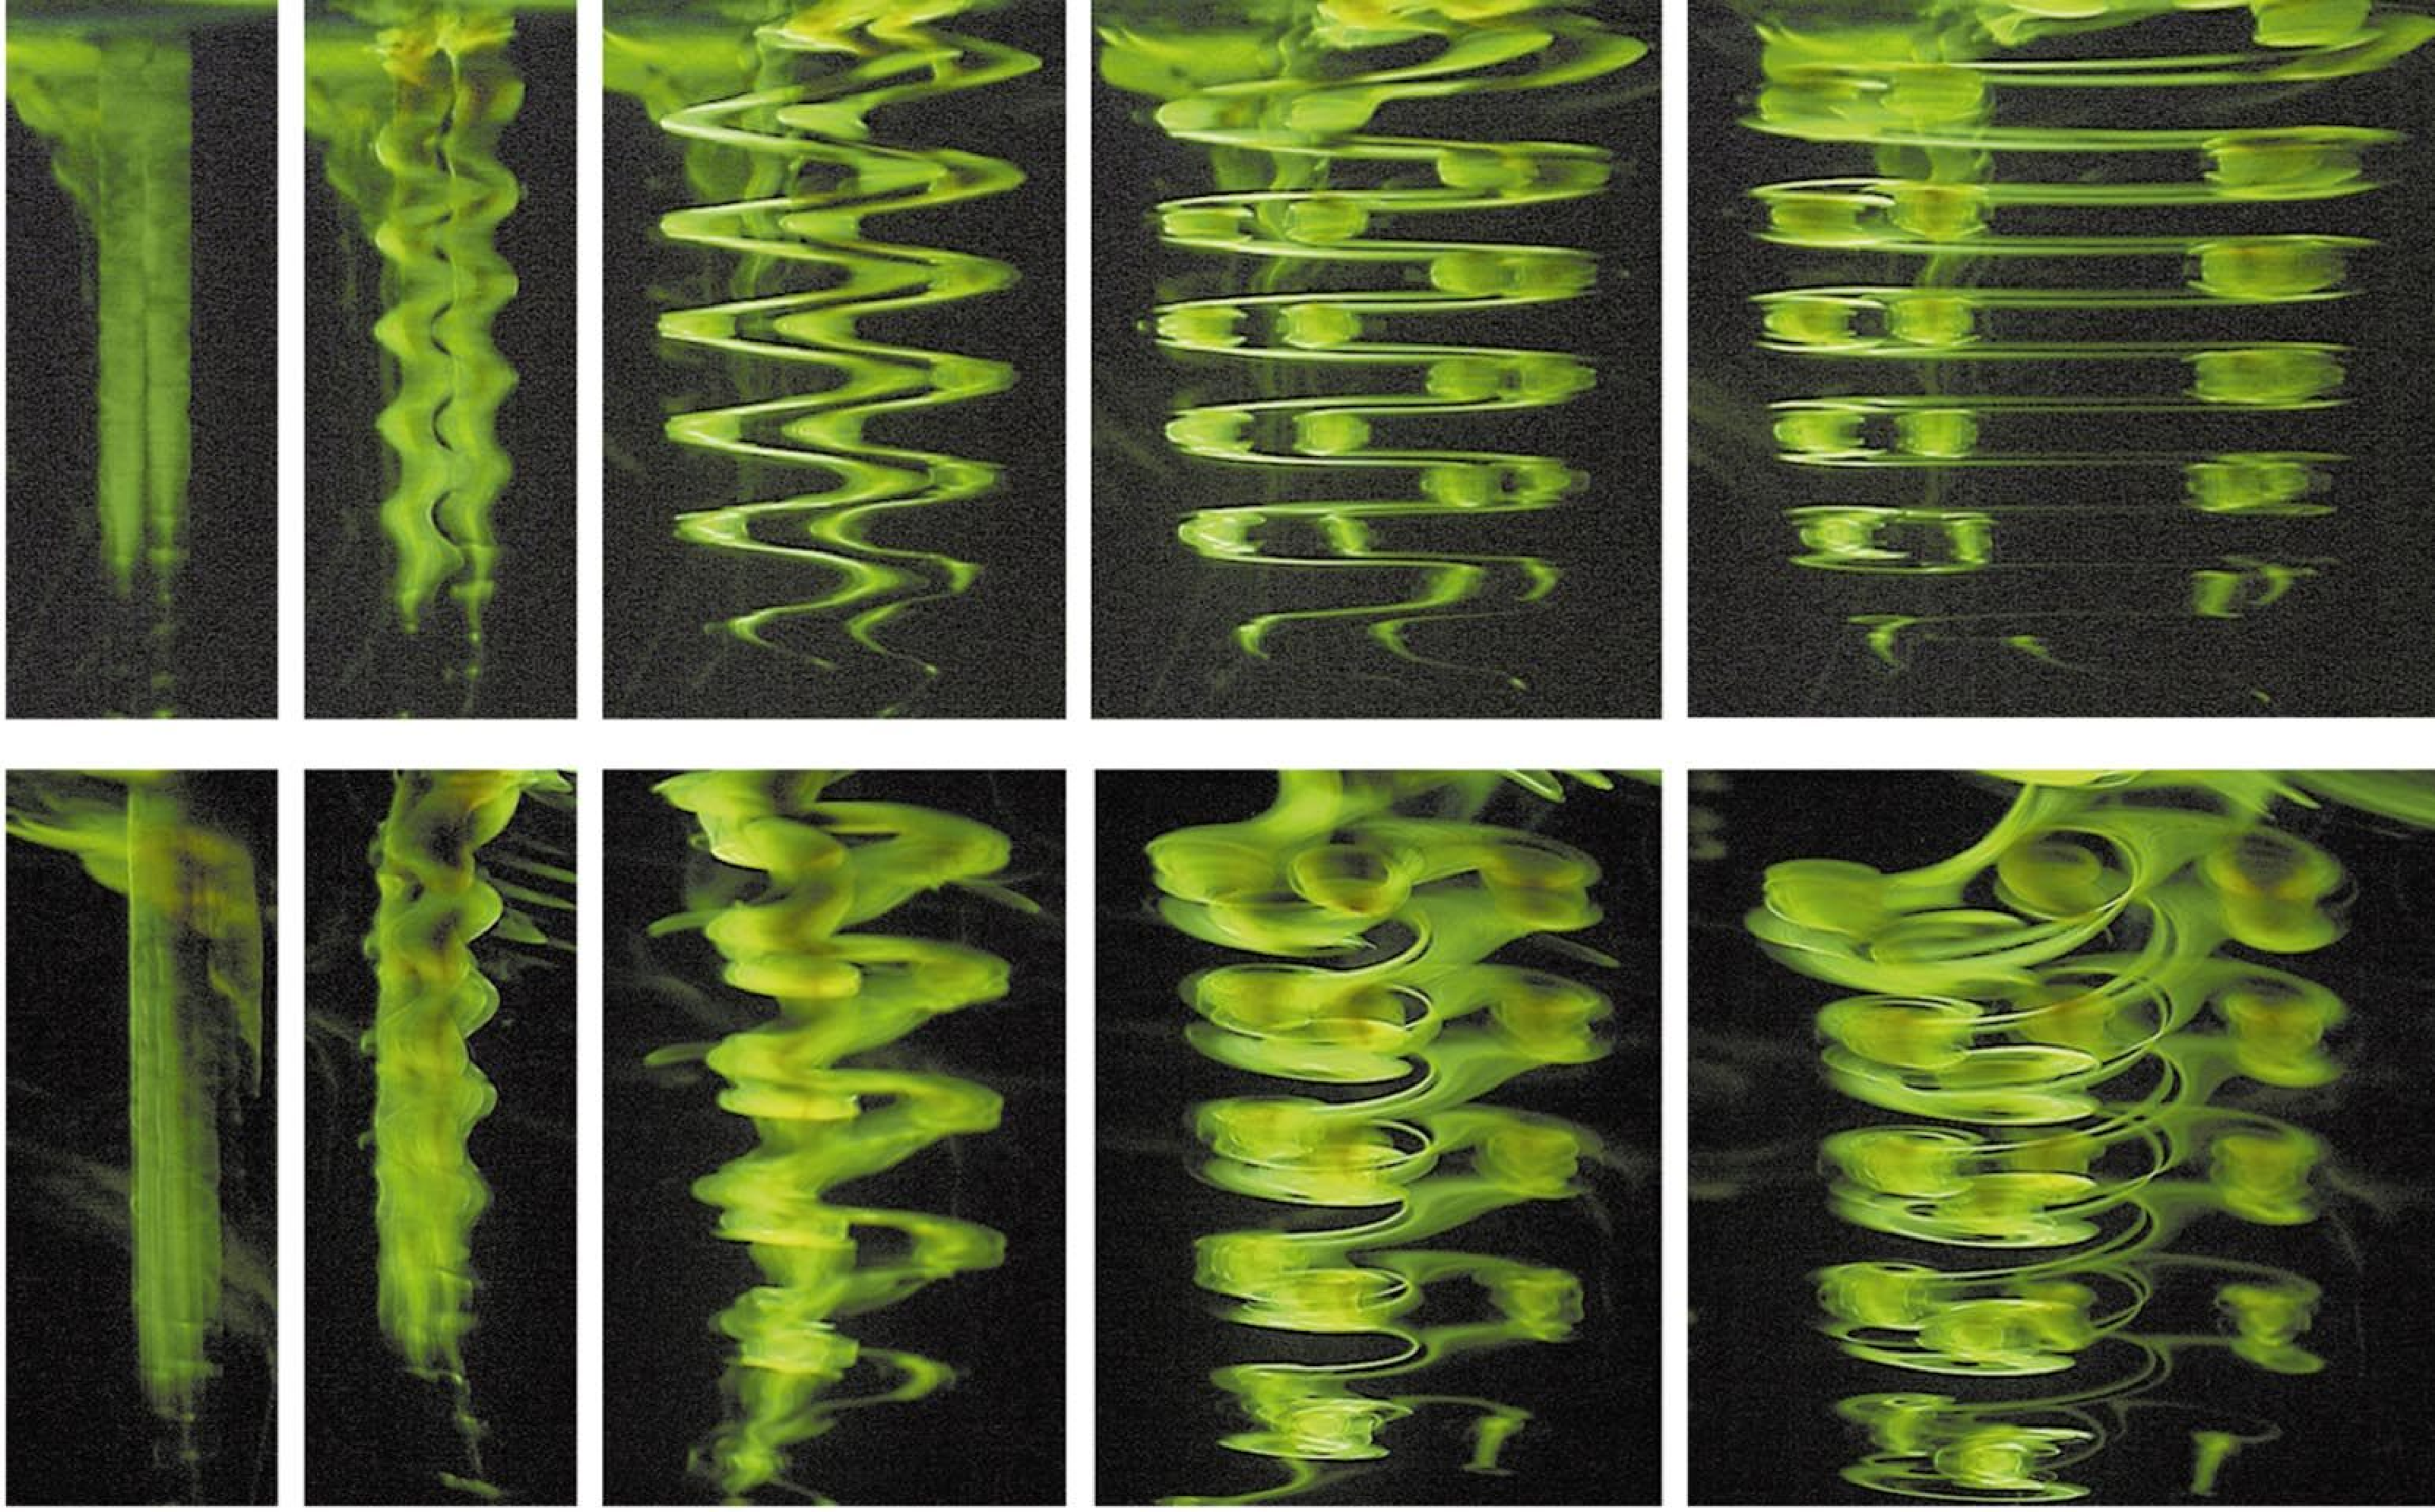
\includegraphics[width=\textwidth]{zigzag_experimental.pdf}
%\caption{(get permission from JFM for picture + caption) A sequence of frontal (top) and side (bottom) views showing the growth of the zigzag instability for $F_{h}=0.19$ and $Re=365$. From left to right the pictures are taken at $7,36,75,109,121,176$ seconds after the flaps have closed. The vortex pair is propogating to the left. In this experiment, tape has been applied to force the the natural wavelength of the instability to produce a clearer result.}
%\label{zigzag_experimental}
%\end{center}
%\end{figure}
Figure 10 of \cite{bc2000a} demonstrates the evolution for the zigzag instability for $F_{h}=0.19$ and $Re=365$. The structure of the vortices displays a zigzag like structure. Additionally, the anisotropy between the vertical and horizontal directions is quite clear. The periodic behaviour of the vortex pair is also evident. 

%BC also confirmed the results of the Japanese guys because they found that below $F_{h}=0.22$ the elliptical instability was suppressed by stratification. 

%Billant and Chomaz had experimentally observed this new instability which occured when $F_{h}<0.22$ 

Following up the experimental work, Billant and Chomaz provided a theoretical account of the zigzag instability starting from the Boussinesq equations \cite{bc2000b}. We will only discuss the main result of the paper as the paper is a very technical and long perturbation analysis. In the paper, they investigated the limit where $F_{h,v} = U/L_{h,v}N \ll 1$ and found that the zigzag motion was accounted for by combination of translation and rotation, which agrees with the experimental observations of \cite{bc2000a}. Additionally, they found that the most unstable vertical length scale of the zigzag instability should behave as $F_{v} \sim \mathcal{O}(1)$, i.e. $L_{v} \sim U/N$. This length is known as the buoyancy length scale (e.g. Waite \cite{waite2011}) and has proven to be a very important length scale in stratified fluid flow, as we shall discuss below. This emergence of the buoyancy length scale in their calculations, however,  should be treated with some care since Billant and Chomaz assumed that $F_{v}\ll 1$ and showed that $F_{v}\sim \mathcal{O}(1)$. 

In the third paper, Billant and Chomaz conducted a numerical linear stability analysis of the zigzag instability \cite{bc2000c}. In this study, they numerically solved the linear Boussinesq equations for the growth rate of the leading eigenmode for specific wavenumbers. We will not discuss the results details of the paper here as their paper forms the basis for much of this thesis and we will re-derive and discuss their results throughout the next three chapters. In the remainder of this chapter we derive the numerical equations that Billant and Chomaz used in \cite{bc2000c} and provide some more background information. In Chapter 3 we introduce and discuss the numerical technique of spectral methods used to solve the numerical equations. In Chapter 4 we extend the analysis of Billant and Chomaz to length scales well below the sub-buoyancy scale of $L_{b}\sim U/N$. 

\section{Formulation of the linear problem}
Following Billant and Chomaz \cite{bc2000c}, we consider the non-dimensional Boussinesq approximation to the Navier-Stokes equations in Cartesian co-ordinates 
\begin{align}
\frac{D\bm{u}}{Dt} = -\nabla p - \rho'\hat{\bm{e}}_{z} + \frac{1}{Re}\nabla^{2} \bm{u},\\
\nabla \cdot \bm{u}=0,\\
\frac{D\rho'}{Dt} -\frac{w}{F_{h}^{2}} = \frac{1}{ReSc}\nabla^{2} \rho',
\end{align}
where we have non-dimensionalised by the characteristic velocity $U$, length $R$, time-scale $R/U$, pressure $\rho_{0}U^{2}$, density $\rho_{0}U^{2}/gR$, and defined $Sc=\nu /D$ as the Schmidt number, where $D$ is the mass diffusivity, $\rho_{0}$ is the background density, and $g$ is the gravitational constant. The Reynolds and horizontal Froude number are as defined above. The buoyancy frequency $N$, and hence the Froude number $F_{h}$, is assumed to be constant. 

In order to investigate the linear growth rate, we proceed as in Section 1.2 and expand the full velocity field as the sum of a basic state and a perturbation state:
\begin{align}
\bm{u} = \bm{u}_{0} + \tilde{\bm{u}},\\
p = p_{0} + \tilde{p},\\
\rho' = \rho'_{0} + \tilde{\rho}'.
\end{align}
The basic is chosen to be the Lamb-Chaplygin dipole which we will now discuss and explain how it provides a convenient theoretical model for the experiment by Billant and Chomaz \cite{bc2000a}.


\subsection{The Lamb-Chaplygin Dipole} 
As the basic state for linear stability analysis we use the Lamb-Chaplygin dipole in a comoving frame \cite{meleshko1994}. This dipole is a solution to the 2D inviscid Euler equations. This basic state is motivated by numerous laboratory experiments\cite{bc2000a,leweke1998}, as discussed above, which demonstrated that a vertically oriented Lamb-Chaplygin dipole is a good approximation to the vortex generated by two flaps closing in a tank of salt-stratified water. The dipole, in cylindrical coordinates, is given by the stream function
\begin{align}
\psi_{0}(r,\theta) = 
\begin{dcases}
-\frac{2}{\mu_{1}J_{0}(\mu_{1})}J_{1}(\mu_{1}r)\sin\theta & r\le 1,\\\label{lc_dipole_sf}
-r\left(1-\frac{1}{r^{2}}\right)\sin\theta & r>1 ,
\end{dcases}
\end{align}
and the corresponding vertical vorticity $\omega_{z0}=\nabla_{h}^{2}\psi_{0}$
\begin{align}
\omega_{z0}(r,\theta) = \
\begin{dcases}
\mu_{1}^{2}\psi_{0}(r,\theta) & r\le 1,\\
0 & r>1,
\end{dcases}
\end{align}
where $J_{0},J_{1}$ are the zero and first order Bessel functions, $\mu_{1}\approx 3.8317$ is the first root of $J_{1}$, and $\nabla_{h}$ is the horizontal Laplacian. The basic state velocity is purely horizontal and is given by $\bm{u}_{h0}=\nabla_{h}\psi_{0}\times\hat{\bm{e}}_{z}$. Recall that in the previous section, Billant and Chomaz found experimentally that $\omega = k^{2}\psi$ where $k=1.15$. Here we have that $\omega_{z0}=\mu_{1}^{2}\psi_{0}$. If we consider the dimensional version, we would have that $k^{2} = \mu_{1}^{2}/R^{2}$ where $R=3.6$ cm. This gives $k^{2} = 1.13 \text{ cm}^{-2}$ which corresponds very well with the experimental value of $1.15$. Fig.~\ref{lamb_dipole_plot} is a plot of the vorticity. 

\begin{figure}
\begin{center}
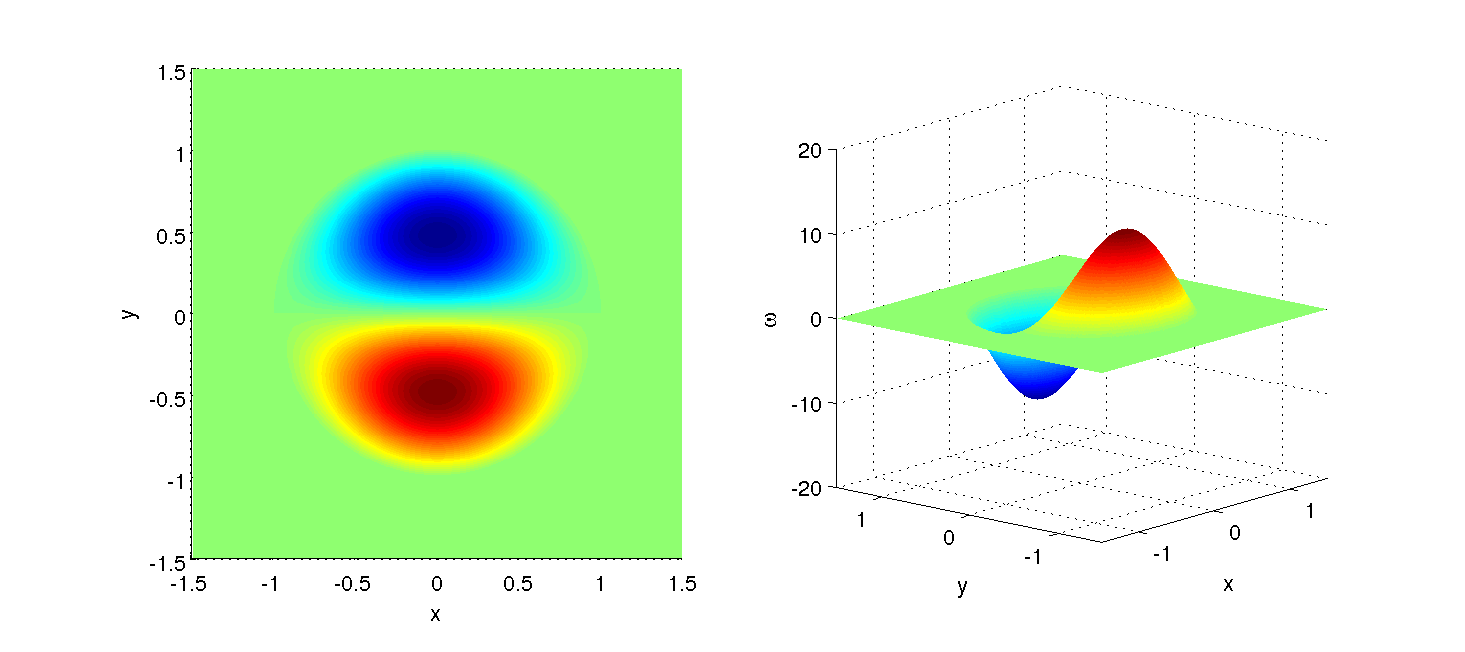
\includegraphics[width=\textwidth]{lamb_dipole}
\caption{The Lamb-Chaplygin dipole.}
\label{lamb_dipole_plot}
\end{center}
\end{figure}
Let us now discuss the derivation of this result, which was first written down by Lamb and investigated further, independently, by Chaplygin \cite{meleshko1994}. Although Lamb was the first to write down the above solution to the Euler equations, he did not provide any motivation for the derivation beyond it being an exact solution of the 2D steady Euler equations. However, a decade later, Lamb provided a slightly more in depth derivation motivating somewhat the study of this dipole. Independently, in Russia, Chaplygin provided a complete derivation and motivation for studying this dipole, although it remained unknown outside of Russia. Following \cite{meleshko1994} we repeat the key points of Chaplygin's argument. 

Recall that the steady 2D Euler equations can be written in terms of the stream function $\psi$ and a vorticity $\omega$ as
\begin{align}
\nabla^{2} \psi = - \omega.\label{vort_eq_chap}
\end{align}
To choose $\omega$, Chaplygin was motivated by the situation where we have a continuous vortex whose outer region is steady irrotational flow while the inner region is a translating vortex. Recall that the potential function for a flow outside a cylinder is
\begin{align}
\psi = v_{0}\left(r - \frac{a^{2}}{r}\right)\sin\theta ,
\end{align}
where $a$ is the radius of the dipole and $v_{0}$ is the propagation velocity. 

Inside the radius $a$, Chaplygin chose the vorticity to be $\omega = n^{2}\psi$ where $n$ is a constant. In polar coordinates (\ref{vort_eq_chap}) becomes
\begin{align}
\frac{\partial^{2}\psi}{\partial r^{2}} + \frac{1}{r}\frac{\partial \psi}{\partial r} + \frac{1}{r^{2}}\frac{\partial^{2}\psi}{\partial \theta^{2}} =  n^{2}\psi,
\end{align}
which we can guess at a solution of the form $\psi(r,\theta) = Z(r)\sin\theta$. Although Chaplygin did not provide specific motivation for choosing this specific vorticity, the above equation has a form that is similar to the irrotational flow outside the dipole and this makes the matching conditions simple. The resulting equation for $Z(r)$ is the well known Bessel equation \cite{meleshko1994} and after working through the algebra, one obtains (\ref{lc_dipole_sf}). Chaplygin also investigated the resulting pressure field produced by the dipole and was able to compute the circulation of the dipole. Unlike Lamb, he also considered a generalisation of the above where the dipole is no longer symmetric about the x-axis. The corresponding vorticity in this case is given by
\begin{align}
\omega = n^{2}(\psi - \lambda),
\end{align}
where $\lambda$ is an arbitrary parameter where $\lambda=0$ is a completely symmetric dipole and $\lambda\rightarrow\infty$ corresponds to a completely asymmetric dipole. Here, again, Chaplygin investigated fully the pressure and circulation produced by this dipole. Additionally, in the same set of papers, Chaplygin also investigated the case of the dipole in rotating fluid, which was independently rediscovered 80 years later. Full details of this derivation are in \cite{meleshko1994}.


\section{Scaling analysis}
We have mentioned two dimensionless numbers in stratified flow, the Reynolds number and the Froude number. Both these dimensionless numbers arise when comparing the relative sizes of various terms in the Navier-Stokes equations. Depending on what aspect of a problem we are looking at, these numbers can appear in different places when we choose different scalings. We will now discuss some of the scaling arguments that have been used in stratified flow as it can provide insights into what mechanisms underlie the transition to and evolution of turbulence. A comprehensive review of scaling in stratified turbulence is provided in a recent review by Riley and Lindborg \cite{rileylindborg2013} and we will discuss the important scaling arguments therein. 

For reference, we reproduce the Boussinesq equations here 
\begin{align}
\frac{\partial \textbf{u}_{h}'}{\partial t'} + \textbf{u}_{h}'\cdot\nabla'_{h}\textbf{u}_{h}'+u_{z}'\frac{\partial \textbf{u}_{h}'}{\partial z'} &= -\frac{1}{\rho_{0}}\nabla'_{h}p' + \nu \nabla'^{2}\textbf{u}_{h},\\
\frac{\partial u_{z}'}{\partial t'} + \textbf{u}_{h}'\cdot\nabla'_{h}u_{z}'+u_{z}'\frac{\partial u_{z}'}{\partial z'} &= -\frac{1}{\rho_{0}}\frac{\partial p'}{\partial z'} - \frac{\rho' g}{\rho_{0}} + \nu \nabla'^{2}u_{z},\\
\nabla'_{h}\cdot\textbf{u}_{h}' + \frac{\partial u_{z}'}{\partial z'} &=0,\\
\frac{\partial \rho'}{\partial t'} + \textbf{u}_{h}'\cdot\nabla_{h}'\rho' + u_{z}'\frac{\partial \rho'}{\partial z'} + \frac{\partial \rho}{\partial z'}u_{z}'&=D\nabla^{2}\rho ',
\end{align}
where the primed quantities denote the dimensional quantities. 

As a starting point, we produce a scaling argument that separates the horizontal and vertical directions. As we saw in the experiment of Billant and Chomaz \cite{bc2000a}, in the zigzag instability there was a clear separation between the vertical and horizontal scales. This difference in the vertical and horizontal directions suggests defining two length scales, the horizontal length scale $L_{h}$ and the vertical length scale $L_{v}$. Associated with this separation we introduce the horizontal velocity scale $U$ and the vertical velocity scale $W$. The resulting scaling is
\begin{align}
x'=L_{h}x,\qquad y' =L_{h}y, \qquad z'=L_{v}z, \qquad \textbf{u}_{h}' = U\textbf{u}, \qquad u_{z}' = Wu_{z}.
\end{align}
We also define another useful quantity that plays an important role in the scaling of stratified flows, the aspect ratio
\begin{align}
\delta = \frac{L_{v}}{L_{h}},
\end{align}
which measures how anisotropic the length scales are. For the time scale, we choose the advective time scale 
\begin{align}
t' = \frac{L_{h}}{U}t,
\end{align}
which is the characteristic time of a vortex to be advected around the characteristic length \cite{rileylelong2000,bc2001,lilly1983}. Following these references the pressure scales such that the horizontal pressure gradient is the same order as the advection terms and density scales from approximate hydrostatic balance
\begin{align}
p' = \rho_{0}U^{2}p, \qquad \rho' = \frac{U^{2}\rho_{0}}{gL_{v}}\rho.
\end{align}
The only quantity left unspecified is the vertical velocity which can be determined by setting balancing the linear terms and the time derivative terms in the density equation \cite{bc2001,rileylelong2000} giving the scaling 
 \begin{align}
u_{z}' = U\frac{F_{h}^{2}}{\delta}u_{z}.
\end{align}
This scaling now leads to the following set of equations \cite{rileylindborg2013}
\begin{align}
\frac{\partial \textbf{u}_{h}}{\partial t} + \textbf{u}_{h}\cdot\nabla_{h}\textbf{u}_{h}+\frac{F_{h}^{2}}{\alpha^{2}}u_{z}\frac{\partial \textbf{u}_{h}}{\partial z} &= -\nabla_{h}p + \frac{1}{\Re}\left(\nabla^{2}_{h}\textbf{u}_{h}+\frac{1}{\alpha^{2}}\frac{\partial^{2}\textbf{u}_{h}}{\partial z^{2}}\right),\\
F_{h}^{2}\left(\frac{\partial u_{z}}{\partial t} + \textbf{u}_{h}\cdot\nabla_{h}u_{z}+\frac{F_{h}^{2}}{\alpha^{2}}u_{z}\frac{\partial u_{z}}{\partial z}\right) &= -\frac{\partial p}{\partial z} - \rho + \frac{F_{h}^{2}}{\Re}\left(\frac{1}{\alpha^{2}}\frac{\partial u_{z}}{\partial z^{2}} + \nabla^{2}_{h}u_{z}\right),\\
\nabla_{h}\cdot\textbf{u}_{h} + \frac{F_{h}^{2}}{\alpha^{2}}\frac{\partial u_{z}}{\partial z} &=0,\\
\frac{\partial \rho}{\partial t} + \textbf{u}_{h}\cdot\nabla_{h}\rho + \frac{F_{h}^{2}}{\alpha^{2}}u_{z}\frac{\partial \rho}{\partial z} &= u_{z} + \frac{1}{\Re Sc}\left(\frac{1}{\alpha^{2}}\frac{\partial^{2}\rho}{\partial z^{2}} + \nabla^{2}_{h}\rho\right),
\end{align} 
where 
\begin{align}
\Re = \frac{UL_{h}}{\nu}, \qquad F_{h} = \frac{U}{L_{h}N},\qquad Sc = \frac{\nu}{D}.
\end{align}
Lilly was the first to write these equations down although he assumed isotropy, i.e. $\delta=1$. 

Let us now investigate the limit of strong stratification, i.e. $F_{h}\rightarrow 0$ but let us leave the behaviour of $F_{h}/\delta$ undetermined. Additionally, let us consider $\Re\gg 1$ and following \cite{rileylindborg2013} ignore the diffusion terms that only depend on $Re$ but not $Re\delta^{2}$.  This results in the following equations 
\begin{align}
\frac{\partial \textbf{u}_{h}}{\partial t} + \textbf{u}_{h}\cdot\nabla_{h}\textbf{u}_{h}+\frac{F_{h}^{2}}{\alpha^{2}}u_{z}\frac{\partial \textbf{u}_{h}}{\partial z} &= -\nabla_{h}p + \frac{1}{\Re}\frac{1}{\alpha^{2}}\frac{\partial^{2}\textbf{u}_{h}}{\partial z^{2}},\\
0&= -\frac{\partial p}{\partial z} - \rho, \\
\nabla_{h}\cdot\textbf{u}_{h}+ \frac{F_{h}^{2}}{\alpha^{2}}\frac{\partial u_{z}}{\partial z} &=0,\\
\frac{\partial \rho}{\partial t} + \textbf{u}_{h}\cdot\nabla_{h}\rho + \frac{F_{h}^{2}}{\alpha^{2}}u_{z}\frac{\partial \rho}{\partial z} &= u_{z} + \frac{1}{\Re Sc}\frac{1}{\alpha^{2}}\frac{\partial^{2}\rho}{\partial z^{2}} .
\end{align} 
It was initially assumed by Lilly \cite{lilly1983} and Riley et al.\cite{rileylelong2000} that as $F_{h}\rightarrow 0$ then so does $F_{h}/\delta$. Thus the resulting equations are 
\begin{align}
\frac{\partial \textbf{u}_{h}}{\partial t} + \textbf{u}_{h}\cdot\nabla_{h}\textbf{u}_{h} &= -\nabla_{h}p + \frac{1}{\Re}\frac{1}{\alpha^{2}}\frac{\partial^{2}\textbf{u}_{h}}{\partial z^{2}},\\
0&= -\frac{\partial p}{\partial z} - \rho  \\
\nabla_{h}\cdot\textbf{u}_{h} &=0\\
\frac{\partial \rho}{\partial t} + \textbf{u}_{h}\cdot\nabla_{h}\rho &= \frac{1}{\Re Sc}\frac{1}{\alpha^{2}}\frac{\partial^{2}\rho}{\partial z^{2}} 
\end{align} 
Notice that in these resulting equations, the horizontal and vertical velocities have become almost completely decoupled. They are not completely decoupled because there is still dependence through the pressure term. However this decoupling led Lilly to conjecture that stratified turbulence in the strong stratification limit will resemble layerwise 2D turbulence with an inverse energy cascade\cite{lilly1983}. However, subsequent numerical simulations of stratified turbulence were not able to reproduce an inverse cascade, raising doubts about the applicability of Lilly's equations (e.g. Herring and Metais \cite{metais1989}, Waite and Bartello \cite{waitebartello2004}).


Building on the work of Lilly \cite{lilly1983} and Riley et al.\cite{rileylelong2000}, Billant and Chomaz \cite{bc2001} modified the argument suggesting that instead $F_{h}/\delta\rightarrow 1$, not $0$, as $F_{h}\rightarrow 1$. This scaling analysis leads to $L_{v} \sim U/N$ which is the dominant vertical scale for the zigzag instability. The resulting equations are

\begin{align}
\frac{\partial \textbf{u}_{h}}{\partial t} + \textbf{u}_{h}\cdot\nabla_{h}\textbf{u}_{h}+u_{z}\frac{\partial \textbf{u}_{h}}{\partial z} &= -\nabla_{h}p + \frac{1}{\Re}\frac{1}{\alpha^{2}}\frac{\partial^{2}\textbf{u}_{h}}{\partial z^{2}},\\
0&= -\frac{\partial p}{\partial z} - \rho, \\
\nabla_{h}\cdot\textbf{u}_{h}+ \frac{\partial u_{z}}{\partial z} &=0,\\
\frac{\partial \rho}{\partial t} + \textbf{u}_{h}\cdot\nabla_{h}\rho + u_{z}\frac{\partial \rho}{\partial z} &= u_{z} + \frac{1}{\Re Sc}\frac{1}{\alpha^{2}}\frac{\partial^{2}\rho}{\partial z^{2}}. 
\end{align} 
The assumption that $F_{h}/\delta \rightarrow 1$ can be rewritten to state that $L_{v} \sim U/N$, which is the buoyancy scale. In this case, there is no decoupling between the horizontal and vertical directions and the advection terms and incompressibility condition are fully three-dimensional. 

\subsection{Stratified Turbulence}
In this thesis we focus on the linear stability and the transition to stratified turbulence, but not on stratified turbulence itself however it worth making a few brief remarks. For an in-depth recent review, see Lindborg and Riley \cite{rileylindborg2013} which contains a thorough review of recent process made in stratified turbulence in experimental, theoretical, and numerical results.

Experimental results by Nastrom and Gage \cite{nastrom1985} analysing data from airplanes have shown that stratified turbulence in the atmosphere exhibits the scaling of the horizontal energy spectrum as $k_{h}^{-3}$ at large horizontal scales and as $k_{h}^{-5/3}$ as small horizontal scales. The $k_{h}^{-3}$ spectrum is well known in the quasi-geostrophic community (source?). The $k_{h}^{-5/3}$ is the well known \cite{lesieur} scaling of isotropic homogeneous turbulence derived by Kolmogorov in the 1940s. The appearance of this scaling is surprising since anisotropy, as we have discussed, is very important in stratified flows. One possible theory, proposed by Lindborg \cite{lindborg2006}, is that the buoyancy length $U/N$, here meaning the length scale of the eddies within the flow, plays the important role in governing the evolution of the turbulence. However many open questions remain (cite?).




%-------------------------------------------------------------------------------
%
%  NUMERICAL STUFF 
%
%-------------------------------------------------------------------------------
\chapter{Numerical Stuff and Introductionary Theory}
\begin{itemize}
\item introduction to the boussinesq approximation 
\item In this section I should introduce the spectral method and the numerical scheme
\item Dealiasing tests 
\item  diffusion test
\item hyperviscosity
\end{itemize}
\section{Boussinesq approximation}

The equations can be written in the dimensional from as (add derivation, Kundu? Batchelor? Others?)

\begin{align}
\frac{\partial \bm{u}}{\partial t} + \bm{u}\cdot \nabla \bm{u} = -\frac{1}{\rho_{0}}\nabla p - \frac{\rho g}{\rho_{0}}\hat{\bm{e}}_{z} + \nu \nabla^{2}\bm{u} \label{boussinesq1}\\
\nabla \cdot \bm{u} =0 \label{boussinesq2}\\
\frac{\partial \rho}{\partial t} + \bm{u}\cdot \nabla \rho = \kappa \nabla^{2}\rho - \frac{\partial \bar{\rho}}{\partial z} w\label{boussinesq3}
\end{align}
where we have the following dimensional variables
\begin{itemize}
\item $\textbf{u}(x,y,z)=(u(x,y,z),v(x,y,z),w(x,y,z))$ is the velocity field in the $x,y,z$-directions directions respectively,
\item $p(x,y,z)$ is the pressure field,
\item $\rho(x,y,z)$ is a perturbation density,
\item $\rho_{0}$ is a constant reference density,
\item $\bar{\rho}$ is ... ? ,
\item $g$ is the gravitational constant,
\item $\nu$ is the constant kinematic velocity ,
\item $\kappa$ is the constant molecular diffusivity.
\end{itemize}
Equations (\ref{boussinesq1})-(\ref{boussinesq3}) are a set of five coupled partial differential equations for the unknowns $\textbf{u},p,\rho$. Herein, we will refer to equation (\ref{boussinesq1}) as the velocity equations, equation (\ref{boussinesq2}) as the continuity equation, and equation (\ref{boussinesq3}) as the density equation. 

Maybe go onto non-dimensionalisation? 

There is a difference between the linear and nonlinear equations (MIke's code uses a slightly modified version of Boussinesq that uses temperature) 
We take the above equations (Ref) as the starting point for our simulations. 

\section{Spectral Methods}
In this thesis we use the spectral method to evaluate the derivatives. Some more background. Spectral methods are based off the following observation. Let us denote the Fourier transform of $f(x)$ as $\hat{f}(k)$, given by
\begin{align}
\hat{f}(k) = \int_{-\infty}^{\infty}dxe^{-ikx}f(x)
\end{align}
Now consider the Fourier transform of the derivative $df/dx$. 
\begin{align}
\int_{-\infty}^{\infty}dxe^{-ikx}\frac{df}{dx}=e^{-ikx}f(x)\bigg|_{-\infty}^{\infty} + ik\int_{-\infty}^{\infty}dxe^{-ikx}f(x)= ik\hat{f}(k)
\end{align}
and thus the Fourier transform of a derivative is just $ik$ times the Fourier transform of $f(x)$. We have assumed here that $f(x)$ vanishes sufficiently quickly at infinity. For most applications of the Fourier transform, this assumption is valid. In this thesis, all functions considered will vanish quickly enough although see section below. (add bit about decay?). In general, it is easy to show that the Fourier transform of $d^{n}f/dx^{n}$ is $(ik)^{n}\hat{f}(k)$. 

Computationally, if we have a quick way to evalute $\hat{f}(k)$ from $f(x)$ and $f(x)$ from $\hat{f}(k)$, then the $n^{\text{th}}$ derivative is easy to compute and results from multiplying by the simple pre-factor $(ik)^{n}$. 

blah blah FFT. Discuss that here.


\section{Dealiasing} 
An important consideration in transforming between physical and Fourier space is the problem of aliasing.

Explain what it is! Blah blah wavenumbers meet and cross and cause problems.

Add derivation from Durran on this.

In the code we use a 2/3s rule however others have used other rules. To determine 

\section{1D Example} 
In this section we demonstrate the differences between solving PDEs in real space vs Fourier space. Consider the following one dimensional wave equation\cite{trefethen_spectral}
\begin{align}
\frac{\partial u}{\partial t} + c(x)\frac{\partial u}{\partial x} = 0,\qquad c(x)=\frac{1}{5}+\sin^{2}(x-1), \qquad u(x,0)=e^{-100(x-1)^{2}}, x\in[0,2\pi], t>0
\end{align}
where we are solving on a periodic domain. The physical interpretation of this equation is the simple one dimensional advection of a velocity field $u(x,t)$ by the fixed field $c(x)$. To illustrate issues relating to the spectral method, we will solve this problem in two ways: first we solve in the physical domain to demonstrate the idea of spectral differentiation and second to solve it in Fourier space to demonstrate the issues of dealiasing.

For a time-stepping scheme, we use a second-order Adams-Bashforth\cite{durran} scheme. Re-writing wave-equation as
\begin{align}
\frac{\partial u}{\partial t} = -c(x)\frac{\partial u}{\partial x} = F(u)
\end{align}
the Adams-Bashforth scheme is
\begin{align}
u^{n+1} = u^{n} + \frac{\dt}{2}[3F(u^{n})-F(u^{n-1})]
\end{align}
Since the Adams-Bashforth scheme uses a previous time-step, we will use forward Euler for the first time-step. To evalute $F(u)$ we will use the spectral differentiation, as discussed above. 
Figures go here.

Now we consider solving the equation in Fourier space. Taking the Fourier transform we obtain
\begin{align}
\frac{\partial \hat{u}}{\partial t} + \widehat{c(x)\frac{\partial u}{\partial x}}=0
\end{align}

\section{Navier-Stokes in Fourier Space}
\subsection{Fourier Transformed Navier-Stokes}
We now turn to the formulation of the Navier-Stokes equations in a Fourier domain. The Fourier domain provides a convenient formulation to analyse the underlying mechanisms of turbulence, as we shall see. Recall that in the Fourier domain, derviatives become multiplcation of wavenumbers which converts the spatial parts of the Navier-Stokes equations into algebraic equations. 

To demonstrate the formulation in Fourier space, let us cast the standard Navier-Stokes equations into Fourier space. 
\begin{align}
\frac{\partial \textbf{u}}{\partial t} + \textbf{u}\cdot\nabla\textbf{u} = -\frac{1}{\rho_{0}}\nabla p + \nu\nabla^{2}\textbf{u}, \qquad \nabla\cdot\textbf{u}=0
\end{align}
Taking the Fourier transform of the above equation is straight-forward for all terms except the advection term $\textbf{u}\cdot\nabla\textbf{u}$, which we postpone for now.

In Fourier space, we can also exploit the following observation to eliminate the pressure term, thus saving the need to solve a Poisson equation at each time-step. The incompressibility condition becomes $\textbf{k}\cdot\hat{\textbf{u}}(\textbf{k},t)=0$ in Fourier space. Geometrically, this means that the vectors $\textbf{k}$ and $\hat{\textbf{u}}$ are orthogonal. To see this define a $\textbf{k}$-plane and a $\hat{\textbf{u}}$-plane. The defining equation of a plane is $ax+by+cz=d$ with the normal vector $\textbf{n}=(a,b,c)$. Here the normal vectors are $\textbf{k}$ and $\hat{\textbf{u}}$. Thus if the normal vectors are orthogonal, the planes are orthogonal.

This realisation tells us that vectors that are proportional to \uhatm are orthogonal to vectors that are proportional to \kvecm. Thus writing out the Navier-Stokes equations
\begin{align}
\frac{\partial \uhat}{\partial t} + \mathcal{F}(\textbf{u}\cdot\nabla\textbf{u}) = -\frac{1}{\rho_{0}} \kvec\hat{p} - \nu k^{2}\uhat\label{NS_fourier_1},
\end{align}
take the dot product with \kvecm and using the orthogonality condition we obtain
\begin{align}
\kvec\cdot\mathcal{F}(\textbf{u}\cdot\nabla\textbf{u}) + \frac{1}{\rho_{0}}k^{2}\hat{p}=0\label{pressure_fourier_1}.
\end{align}
Isolating for pressure and substituting back into (\ref{NS_fourier_1}) we obtain
\begin{align}
\frac{\partial \uhat}{\partial t} + \mathcal{F}(\textbf{u}\cdot\nabla\textbf{u})(\textbf{1}-\frac{\kvec\kvec}{k^{2}})= - \nu k^{2}\uhat\label{NS_fourier_2}.
\end{align}
This result is unsurprising, since all we have done is take the divergence of the Navier-Stokes equations, which in Fourier space corresponds to taking the dot product with respect to $\kvec$. But using this observation we can avoid the need for solving the pressure altogether because the pressure term is orthogonal to the $\uhat$-plane. But what about the advection term? As can be seen in (\ref{NS_fourier_2}), it has this factor $\textbf{1} - \kvec\kvec/k^{2}$ multiplying it. This term represents a projection into the $\uhat$-plane. The advection term can thought of a vector that is pointing in some direction inbetween the planes of $\kvec$ and $\uhat$. By projecting the advection term into the $\uhat$-plane, we would have a set of equations that are independent of the pressure completely.

\subsection{Projection Tensor}
In order to project the Navier-Stokes equations onto the $\uhat$-plane, we define the following projection operator
\begin{align}
\textbf{P}=\textbf{1} - \frac{\kvec\kvec}{k^{2}} = P_{ij}(\kvec) = \delta_{ij} - \frac{k_{i}k_{j}}{k^{2}}
\end{align}
where we are using Einstein summation notation \cite{lesieur,wald}. It is straight forward to verify that $P_{ij}P_{jk}=P_{ik}$ or in matrix notation $\textbf{P}^{2}=\textbf{P}$, in other words the projection tensor is idempotent. Idepotence is a defining feature of projection operators \cite{MeyerLinAlg}. It is straightforward to verify that $k_{j}P_{ij}=0$ and $\hat{u}_{j}P_{ij}=\hat{u}_{i}$. These simple observations confirm that the projection tensor projects a vector onto the $\uhat$-plane. 

Applying $P_{ij}$ to (\ref{NS_fourier_1}) we obtain the following 
\begin{align}
\frac{\partial \uhat}{\partial t} + \textbf{P}\mathcal{F}(\textbf{u}\cdot\nabla\textbf{u}) =  -\nu k^{2}\uhat\label{NS_fourier_2}
\end{align}
where $\textbf{P}$ is acting on the Fourier transform of the advection term. In order to compute the Fourier transform of the advection term, we note that 
\begin{align}
\textbf{u}\cdot\nabla\textbf{u} = u_{j}\frac{\partial u_{i}}{\partial x_{j}} = \frac{\partial (u_{i}u_{j})}{\partial x_{j}}
\end{align}
where the incompressibility condition has been used to bring the velocity inside the derivative. Thus we are able to write
\begin{align}
\mathcal{F}(\textbf{u}\cdot\nabla\textbf{u})=ik_{j}\int_{\textbf{p}+\textbf{q}=\kvec}d\kvec\hat{u}_{i}(\textbf{p})\hat{u}_{j}(\textbf{q})
\end{align}
and hence we can finally write out the Navier-Stokes equations in Fourier space as \cite{lesieur}
\begin{align}
\frac{\partial \hat{u}_{i}}{\partial t} + iP_{ij}k_{m}\int_{\textbf{p}+\textbf{q}=\kvec}d\kvec\hat{u}_{j}(\textbf{p})\hat{u}_{m}(\textbf{q})=  -k^{2}\hat{u}_{i}\label{NS_fourier_3}
\end{align}

\subsection{Numerical Formulation of NS in Fourier}
Although we have eliminated the pressure completely, we still have an integral term in the equation. To formulate this problem numerically, we make the following observation that is useful in spectral methods \cite{lesieur,orszag1972}.

Recall the following identity (Kundu, Acheson)
\begin{align}
\textbf{u}\cdot\nabla\textbf{u} = \bm{\omega}\times \textbf{u} - \frac{1}{2}\nabla \textbf{u}^{2}
\end{align}
When we apply the projection operator $\textbf{P}$ to the above equation, the $\nabla \textbf{u}^{2}$ term will vanish since it is orthogonal to the $\uhat$-plane. For the cross product between the vorticity and velocity, we use the methods discussed above from dealiasing. Thus to evaluate the cross product term, we assume we have the Fourier transform of the vorticity and velocity $\hat{\bm{\omega}},\uhat$ and re-write the cross product term as
\begin{align}
\mathcal{F}(\bm{\omega}\times \textbf{u}) = \mathcal{F}(\mathcal{F}^{-1}(\hat{\bm{\omega}})\times\mathcal{F}^{-1}(\uhat))
\end{align}
Using this result we can reformulate the Navier-Stokes equations into a form to be solved numerically using a spectral method
\begin{align}
\frac{\partial \uhat}{\partial t} = \textbf{P}(\kvec)\mathcal{F}(\mathcal{F}^{-1}(\hat{\bm{\omega}})\times\mathcal{F}^{-1}(\uhat))-k^{2}\uhat
\end{align}
where the $\mathcal{F},\mathcal{F}^{-1}$ can be evaluated by FFTs, as discussed above.

This reformulation of the Navier-Stokes equations into Fourier space simplifies numerical calculations immensely and provides many advantages over the real space formulation. The absence of the pressure term means that there is no Poisson equation to be solved at each time-step for the pressure. If one did want the pressure, one can solve (\ref{pressure_fourier_1}) for $\hat{p}$. In addition there is no need to enforce a divergence free solution\footnote{Except possibily at the initial time step, see Section 3.} as the equations are formulated by definition to satisfy divergence free condition. The only additional technical difficulty is evaluating the vorticity, but this can easily be handled because of the simple structure of the curl. 

\subsection{Integrating Factor}
Another advantage of the Fourier formuation is the ability to exactly integrate the diffusion term. Let us denote the advective projective term as $F(\hat{u})$ and we have
\begin{align}
\frac{\partial \uhat}{\partial t} + \nu k^{2}\uhat = F(\uhat) 
\end{align}
where the left-hand side has been explicitly written out. Written in this form, the common trick of writing a product as a derivative is observed since
\begin{align}
 \frac{\partial \uhat}{\partial t} + \nu k^{2}\uhat= e^{-\nu k^{2}t}\frac{\partial \uhat e^{\nu k^{2}t}}{\partial t} 
\end{align}
Thus we can re-write the Navier-Stokes equations as 
\begin{align}
\frac{\partial \uhat e^{\nu k^{2}t}}{\partial t} = e^{\nu k^{2}t}F(\uhat)
\end{align}
For notational convenience, let us write that $g(t) = e^{\nu k^{2}t}$ and the note the following trivial identities
\begin{align}
g(t\pm\dt) = g(t)g(\pm\dt),\qquad g(0) = 1, \qquad g(t)^{-1} = g(-t).\label{int_fact_ident}
\end{align}
With this notation the Navier-Stokes equations become
\begin{align}
\frac{\partial (\uhat g(t))}{\partial t} = g(t)F(\uhat).
\end{align}
 Now let us solve the above system using an Adams-Bashforth 2nd order time-stepping scheme. Initially we obtain
\begin{align}
\uhat^{n+1}g(t_{n}+\dt) = \uhat^{n}g(t_{n}) + \frac{3}{2}\dt g(t_{n})F(\uhat^{n}) - \frac{1}{2}\dt g(t_{n-1})F(\uhat^{n-1}).
\end{align}
Using the identities in (\ref{int_fact_ident}) the scheme reduces to
\begin{align}
\uhat^{n+1} = g(-\dt)\uhat^{n} + \frac{3}{2}\dt g(-\dt)F(\uhat^{n}) - \frac{1}{2}\dt g(-2\dt)F(\uhat^{n-1}),
\end{align}
and the diffusion term has been reduced to a multiplication by a constant factor $g(-\alpha\dt)$.

\subsection{Hyperviscosity}
blah blah hyperviscosity

\subsection{Concluding Remarks (rename)}
Although we have done all our manipulations in Fourier space, we could have equally well formulated the above equations in real space. The idea of projecting the velocity field onto the $\uhat$-plane is motivated by the Helmholtz decomposition. This decomposition states, for any $C^{2}$ vector field in a bounded region of $\mathbb{R}^{3}$, we can decompose the vector field into a divergence-free and curl-free component. The divergence free part corresponds to taking the divegence of the Navier-Stokes equations which would yield the Poisson equation for the pressure. Taking the curl of the Navier-Stokes equation - which we define to be the vorticity - would yield the vorticity equation which does not have a pressure term. 



%-------------------------------------------------------------------------------
%
%   LINEAR THEORY 
%
%-------------------------------------------------------------------------------
\chapter{Linear Theory}

\section{Introduction and Motivation}
The stability of flows has a long and rich history within fluid dynamics. The classic experiment into the stability of fluid flow is that of  Reynolds \cite{reynolds1883}. In this experiment, Reynolds injected dye into the laminar flow through a pipe. By varying the velocity of the flow through the pipe. If the velocity was sufficiently low, Reynolds was able to observe ``a beautiful straight line through the tube". At slightly higher velocities, the straight line behaviour remained near the initial part of the pipe but further down ``the streak would shift about the tube, but there was no appearance of sinuosity". By increasing the velocity significantly, the dye would again initially remain straight near the initial part of the tube, but instead of shifting about the tube "the colour band would all at once mix up with the surrounding water, and fill the rest of the tube with a mass of coloured water". 

What Reynolds observed was the transition and breakdown of a flow into turbulence. Through careful observation, he determined that the dimensionless quantity that governed the behaviour of the flow was the Reynolds number 
\begin{align}
Re =\frac{UL}{\nu},
\end{align}
a number which, as discussed above represents the ratio between the inertial and viscous terms in the Navier-Stokes equations. Reynolds found that if $Re<13000$ then the flow would remain stable. The natural question to ask is to whether we can predict such numbers analytically or numerically. Due to the complex of the Navier-Stokes equations, a simplying approach must be derived. In order to do this, consider the following idea. Let $\bm{u}_{0}$ denote a basic state that solves the Navier-Stokes equations and let $\bm{u}'$ denote a small unknown perturbation such that $|\bm{u}'|\ll |\bm{u}_{0}|$. Mathematically this means
\begin{align}
\bm{u}(x,t) = \bm{u}_{0}(x,t) + \bm{u}'(x,t).\label{linear_def}
p(x,t) = p_{0}(x,t) + p'(x,t)
\end{align}
Now let us plug (\ref{linear_def}) into the Navier-Stokes equations and expand
\begin{align}
\frac{\partial \bm{u}_{0}}{\partial t} + \frac{\partial \bm{u}'}{\partial t} + (\bm{u}_{0}+\bm{u}')\cdot\nabla(\bm{u}_{0}+\bm{u}') = -\frac{1}{\rho_{0}}\nabla(p_{0} + p') + \nu\nabla^{2}(\bm{u}_{0} + \bm{u}')\\\label{expanded_lin_NS}
\nabla \cdot \bm{u}_{0} + \nabla \cdot \bm{u}'=0.
\end{align} 
Expanding out the advection term yields
\begin{align}
 (\bm{u}_{0}+\bm{u}')\cdot\nabla(\bm{u}_{0}+\bm{u}') &= \bm{u}_{0}\cdot\nabla\bm{u}_{0} + \bm{u}_{0}\cdot\nabla \bm{u}' + \bm{u}'\cdot\nabla\bm{u}_{0} + \bm{u}'\cdot\nabla\bm{u}'\\
&= \bm{u}_{0}\cdot\nabla\bm{u}_{0} + \bm{u}_{0}\cdot\nabla \bm{u}' + \bm{u}'\cdot\nabla\bm{u}_{0} + \mathcal{O}(\bm{u}'^{2})
\end{align}
where we have written the $\bm{u}'\cdot\nabla\bm{u}'$ term has $\mathcal{O}(\bm{u}'^{2})$ because this term is of order $\bm{u}'$ squared, which we assume to be small. Now recall that the basic state $\bm{u}_{0}$ solves the Navier-Stokes equations. Thus in (\ref{expanded_lin_NS}) there are terms that depend just on $\bm{u}_{0}$ and they will vanish by definition of it being a solution to the Navier-Stokes equations. Thus we now have that
\begin{align}
\frac{\partial \bm{u}'}{\partial t} + \bm{u}_{0}\cdot\nabla \bm{u}' + \bm{u}'\cdot\nabla\bm{u}_{0} + \mathcal{O}(\bm{u}'^{2})  = -\frac{1}{\rho_{0}}\nabla p' + \nu\nabla^{2}\bm{u}'\\
 \nabla \cdot \bm{u}'=0.
\end{align}
So far, the equation above is exact and we have just supressed the quadratic nonlinear term in the Big-O notation. Now the critical assumption we make is that because $\bm{u}'$ is small relative to the basic state, $\bm{u}'^{2}$ is even smaller thus is negligible. In other words, we are throwing away the quadratic nonlinearity of the perturbation term because it assumed to be small. 

This is an important point that can be sometimes lost in linear stability analysis. Since we are explicitly assuming that $|\bm{u}'|\ll |\bm{u}_{0}|$ the above equations are only valid when this is the case. As we shall see in numerical simulations, this assumption is not necessarily valid at all times. (Expand this a bit in terms of an energy discussion).

Now making the approximation that $\mathcal{O}(\bm{u}'^{2})$ is small we obtain
\begin{align}
\frac{\partial \bm{u}'}{\partial t} + \bm{u}_{0}\cdot\nabla \bm{u}' + \bm{u}'\cdot\nabla\bm{u}_{0} =  -\frac{1}{\rho_{0}}\nabla p' + \nu\nabla^{2}\bm{u}'\\
 \nabla \cdot \bm{u}'=0.
\end{align}
The above set of equations is linear which means they are more amenable to analytical techniques. 

To demonstrate an example of the general idea of linear stability, we will discuss the formulation of the experiment of Reynolds. This is a standard example and we follow the derivation of \cite{drazinreid}. It will also elucidate the key features of linear stability analysis that we will use below. 

The first simplifying assumption we make is that the basic state $\bm{u}_{0}=U(z)\hat{\bm{e}}_{x}$, a parallel shear flow, which simplifies the above equations to
\begin{align}
\frac{\partial \bm{u}'}{\partial t} + U\frac{\partial \bm{u}}{\partial x} + w'\frac{dU}{dz}\hat{\bm{e}}_{x}= -\frac{1}{\rho_{0}}\nabla p' + \nu\nabla^{2} \bm{u}'\\
\nabla \cdot\bm{u}'=0.
\end{align}
If we had considered the Euler equations instead of the Navier-Stokes equations, we would have the same equations as above except with $\nu=0$. Despite this seemingly simple modification, the resulting equation is very different. When the invsicid equations are considered, there are many elegant results that can be derived for the special case of parallel shear flow without specific what parallel shear flow we are considering. For example, the Rayleigh's inflection point theorem states that a necessary condition for instability is that the basic velocity profile should have an inflection pointer\cite{drazinreid}. A complete discussion of this result and others can be found in \cite{drazinreid,kundu}.

The next step is to expand the above solutions as Fourier modes (add more justification)
\begin{align}
\bm{u}'(x,t) = \hat{\bm{u}}(z)e^{i(\alpha x +\beta y -\alpha ct)}\\
p'(x,t) = \hat{p}(z)e^{i(\alpha x +\beta y -\alpha ct)}
\end{align}
where we take the real part of the above solutions. We require that the solution remainds bounded as $x,y\Rightarrow\pm\infty$ which means that $\alpha,\beta$ must remain real. For $c$, however, we let it remain an arbitrary complex number $c=c_{r} + ic_{i}$. Depending on the sign of $c_{i}$ the result will either decay or grown exponentially as time goes to infinity. We thus associate stability with $c_{i}\le 0$ and instability with $c_{i}>0$. Hence, if we are able to solve the above system and derive a criteria for the value of $c_{i}$ we will be able to derive some criteria for the stability of the flow.

Plugging in the above Fourier expansions into the linaer equations would yield an eigenvalue-eigenvector problem with $\alpha,\beta,c,Re$ being undetermined. From there we could apply numerical linear algebra routines to solve numerically for various $Re,\alpha,\beta$ and obtain a stability curve for $c$. However, a result due to Squire allows us to simplify the problem significantly. Squire's theorem states that to obtain the minimum critical Reynolds number it is sufficient to cosndier only two-dimesnional disturbances\cite{drazinreid}. In other words, for every three dimensional mode, there is a more unstable two dimensional eigenmode. A proof is provided in \cite{drazinreid}. 

Because we only need to consider two dimensional flow, the unknown velocity $\bm{u}'$ can be rewritten in terms of the stream function $\psi'(x,y,z,t)$. Another advantage of writing the equations in terms of the stream function is that the pressure is eliminated, as discussed in the previous sections, further reducing the number of unknowns. 

Denoting $\hat{\phi}$ as the amplitude of the stream function, the linear equations can be re-written as a single equation
\begin{align}
(D^{2}-\alpha^{2})^{2}\phi = (i\alpha \Re)(U-c)(D^{2}-\alpha^{2})\phi -(i\alpha \Re)U''\phi
\end{align}
along with the appropriate boundary conditions. This equation is known as the Orr-Sommerfeld equation and has a rich history in the development of fluid mechanics. A comprehensive review of the various methods of solving this equation, WKB theory, asymptotics, perturbation theory, and so, is contained in \cite{drazinreid} (van Dyke). 

This simple derivation has resulted in a single equation with three unknowns $\alpha,c,Re$ and by choosing different $Re$ and $\alpha$, we can determine a criteria for $c$. Although much work has been done at the beginning of the 20th century to derive approximate solutions to the Orr-Sommerfeld equation, numerically it is very easy to solve. We can reformulate the above equation as a generalised eigenvalue problem for a given parallel shear flow and solve the problem rather easily on a computer. (rewrite) (add Trefethen and some bits on how it relates Orr)

This example motivates the technique of linear stability. Here we have studied the Navier-Stokes equations directly instead of, the perhaps more promising, Euler equations. Recall the Euler equations arise by setting the viscosity to $0$ or letting the Reynolds number go to infinity. In the full blown problem of turbulence, a high Reynolds number on the order of $10^{8}-10^{9}$ is typical and since the inverse of the Reynolds number appears in front of the diffusion term, it seems reasonable to instead ignore the diffusion term since the coefficient is $\mathcal{O}(\Re^{-1}) \ll 1, Re\gg 1$. This would be a mistake. This is because the limit $Re\rightarrow\infty$ is a singular limit. Consider the following simplified model which arises in the study of boundary layers of shear bounded wall flow\cite{benderorszag,acheson_fluid,kundu}
\begin{align}
\epsilon y'' - y =0 \qquad y(0)=0,\qquad y(1)=1.
\end{align}
If we set $\epsilon=0$ we would obtain the equation 
\begin{align}
- y =0 \qquad y(0)=0,y(1)=1.
\end{align}
which clearly has no solution that satisfies the boundary conditions. If we tried a perturbation expansion of the form $y(x) =\sum_{n=0}y_{n}(x)\epsilon^{n}$ we would get nowhere because the lowest order term does not exist. If we solve the full equation, we see the problem with setting $\epsilon=0$,
\begin{align}
y(x) = \frac{e^{x/\epsilon}-1}{e^{1/\epsilon}-1}.
\end{align}
In this equation, we cannot set $\epsilon=0$ because that results in a singular limit. Thus regardless of how small we choose $\epsilon$, there will be a thin layer, called the boundary layer, which is essential to the fluid flow. For a discussion of techniques in singular perturbation theory in terms of the linear stability of the Navier-Stokes equations see \cite{drazinreid}.


\section{A Brief History of Vortex Instabilties}

The origin of vortex instabilities begins with Lord Kelvin who in 1880 studied perturbations to columnar vortices and determined that they were stable. For the next hundred or so years, the theory of vortex instability was quiet until the field was re-ignited by the investigations Crow\cite{crow1970}. Motivated by engineering applications, Crow was an aeronautical engineer, he discovered that for long wavelength perturbations of a pair of counter-rotating vortices that there was a symmetric deformation of the vortices. This worked extended a few years later by Widnall et. al \cite{widnall1974} to small wavelength perturbations. Further investigations into small wavelength perturbations were carried out by numerous others\cite{moore1975,tsai1976} (add in ref 3-7 bc1999) however these studies only considerd vortex filaments (define). It was noticed in these studies that the streamlines of the vortex became elliptical. Following through, Pierrehumbert\cite{pierrehumbert1986} investigated the simple case of a single 2D vortex subject to a constant 3D pertubation. Further work was done by Bayly \cite{bayly1986} and Waleffe\cite{waleffe1990}.

Something about the work of the japanese guys + experimental results. 

A complete and detailed history of the elliptical instability, including derivations and results of the above papers and nonlinear investigations, is presented in the review by Kerswell\cite{kerswell2002}.
\section{Zigzag Instability}
Motivated by the work above (cite), Billant and Chomaz investigate experimentally\cite{bc2000a}, theoretically\cite{bc2000b}, and numerically \cite{bc2000c} the evolution of a apair of columnar vortices in a stratified tank.

First Billant and Chomaz investigated the zigzag instability experimentally. To do this, they investigated a columnar vortex pair in a stratified fluid and investigated the evolution of the resulting flow. We now briefly discuss their experimental procedure since it provides important motivation for the resulting numerical study. 

In order to study the effects of stratification on the evolution of vortices, they first needs to create the vortices. To do this, they used a pair of motor-controlled flaps whose initial angle and closing time could be controlled precisely by a computer. When the flaps were closed, a pair of counter-rotating vortices was produced. They found that the important determining factor in the creation of the vortices was the angle of the flaps. If the angle was too small, additional vortices created when the flaps finally stopped closing were being advected by the dipole and causing spurious instability. For large angles fluid that was initially inbetween the flaps was being injected in the flow and again causing spurious oscillations. In order to balance out these effects, an angle of $14^{\circ}$ was chosen. After fixing the seperation angle they found that by varying the closing time of the flaps, the velocity of the pair of vortices could be changed. Interestingly, the decay of the vortices, roughly $90$s, was independent of the closing time of the flaps. This variation in the velocity determined the experimental parameters for the experiment.

The two important dimensional parameters in this experiment were the horizontal Froude number 
\begin{align}
F_{h} = \frac{U}{NR}
\end{align}
and the Reynolds numbers
\begin{align}
\Re= \frac{UR}{\nu}
\end{align}
where $U$ is the propagating velocity of the dipole as above, $R$ is the riadus of the dipole, $\nu$ is the viscosity of the tank, and $N$ is the buoyancy frequency. Here the viscosity $\nu$ and the radius $R$ were fixed by experimental conditions and could not be varied. Thus the only parameters that could be varied were $N$ and $U$. Since the Froude number was more difficult to vary, as changing it required draining and refilling the tank, the velocity was the only parameter that could be reasonably varied. Since $U$ shows up in both dimenionless numbers, changing $U$ resulted in the changing of both numbers, i.e. they are directly related by the following relationship
\begin{align}
\Re = F_{h}\frac{NR^{2}}{\nu}
\end{align}

To determine a theoretical model of the dipole, they computed the FFT of the measured vorticity in order to determine the streamfunction. They found that there was a linear fit between the vorticity $\omega$ and the streamfunction $\psi$ such that $\omega = -k^{2}\psi$ where $k^{2}=1.15$ which, as we will show below, corresponds to a Lamb-Chaplygin dipole. 

Add in result about using tape to excite most important mode and vertical orientation. 

A discussion of the theoretical paper will go here.

A discussion of the numerical paper will go here.


\section{Formulation of Problem}
We consider the non-dimensional Boussinesq approximation to the Navier-Stokes equations in Cartesian co-ordinates (ref from intro)
\begin{align}
\frac{D\bm{u}}{Dt} = -\nabla p - \rho'\hat{\bm{e}}_{z} + \frac{1}{Re}\nabla^{2} \bm{u},\\
\nabla \cdot \bm{u}=0,\\
\frac{D\rho'}{Dt} -\frac{w}{F_{h}^{2}} = \frac{1}{ReSc}\nabla^{2} \rho',
\end{align}
where $D/Dt=\partial/\partial t + \bm{u}\cdot \nabla, \bm{u}=(u,v,w)$ is the velocity, $p$ is the pressure, and $\rho'$ is the density perturbation. We have non-dimensionalised by the characteristic velocity $U$, length $R$, time-scale $R/U$, pressure $\rho_{0}U^{2}$, density $\rho_{0}U^{2}/gR$, and defined $Sc=\nu /D$ as the Schmidt number, where $D$ is the mass diffusivity, $\rho_{0}$ is the background density, and $g$ is the gravitational constant. The Reynolds and horizontal Froude number are as defined above. The buoyancy frequency $N$, and hence the Froude number $F_{h}$, is assumed to be constant. 

In order to investigate the linear growth rate, we proceed as the introduction and expand the full velocity field as the sum of a basic state and a perturbation state. 
\begin{align}
\bm{u} = \bm{u}_{0} + \tilde{\bm{u}}\\
p = p_{0} + \tilde{p}\\
\rho' = \rho'_{0} + \tilde{\rho}' 
\end{align}
here the basic state is the Lamb-Chaplygin dipole from above. 


\subsection{The Basic State} 
As the basic state for linear stability analysis we use the Lamb-Chaplygin dipole in a comoving frame \cite{meleshko1994}. This dipole is a solution to the 2D inviscid Euler equations. This basic state is motivated by numerous laboratory experiments\cite{bc2000a,leweke1998}, as discussed above, which demonstrated that a vertically oriented Lamb-Chaplygin dipole is a good approximation to the vortex generated by two flaps closing in a tank of salt-stratified water. The dipole, in cylindrical coordinates, is given by the stream function
\begin{align}
\psi_{0}(r,\theta) = 
\begin{dcases}
-\frac{2}{\mu_{1}J_{0}(\mu_{1})}J_{1}(\mu_{1}r)\sin\theta & r\le 1,\\\label{lc_dipole_sf}
-r\left(1-\frac{1}{r^{2}}\right)\sin\theta & r>1 ,
\end{dcases}
\end{align}
and the corresponding vertical vorticity $\omega_{z0}=\nabla_{h}^{2}\psi_{0}$
\begin{align}
\omega_{z0}(r,\theta) = \
\begin{dcases}
\mu_{1}^{2}\psi_{0}(r,\theta) & r\le 1,\\
0 & r>1,
\end{dcases}
\end{align}
where $J_{0},J_{1}$ are the zero and first order Bessel functions, $\mu_{1}\approx 3.38317$ is the first root of $J_{1}$, and $\nabla_{h}$ is the horizontal Laplacian. The basic state velocity is purely horizontal and is given by $\bm{u}_{h0}=\nabla_{h}\psi_{0}\times\hat{\bm{e}}_{z}$.

Let us now discuss the derivation of this result, which was first written down by Lamb and investigated further, independently, by Chaplygin. Although Lamb was the first to write down the above solution to the Euler equations, he did not provide any motiviation for the derivation beyond it being an exact solution of the 2D steady Euler equations. However, a decade later, Lamb provided a slightly more in depth derivation motivating somewhat the study of this dipole. Independently, in Russia, Chaplygin provided a complete derivation and motivation for studying this dipole, although it remained unknown outside of Russia. Following \cite{meleshko1994} we repeat the key points of Chaplygin's argument. 

Recall that the steady 2D Euler equations can be written in terms of the streamfunction $\psi$ and a vorticity $\omega$ as
\begin{align}
\nabla^{2} \psi = - \omega.\label{vort_eq_chap}
\end{align}
To choose $\omega$, Chaplygin was motivated by the situation where we have a continuous vortex whose outer region is steady irrotational flow while the inner region is a translating vortex. Recall that the potential function for a flow outside a cylinder is
\begin{align}
\psi = v_{0}\left(r - \frac{a^{2}}{r}\right)\sin\theta ,
\end{align}
where $a$ is the radius of the dipole and $v_{0}$ is the propogation velocity. 

Inside the radius $a$, Chaplygin chose the vorticity to be $\omega = n^{2}\psi$ where $n$ is a constant. In polar coordinates (\ref{vort_eq_chap}) becomes
\begin{align}
\frac{\partial^{2}\psi}{\partial r^{2}} + \frac{1}{r}\frac{\partial \psi}{\partial r} + \frac{1}{r^{2}}\frac{\partial^{2}\psi}{\partial \theta^{2}} =  n^{2}\psi
\end{align}
which we can guess at a solution of the form $\psi(r,\theta) = Z(r)\sin\theta$. Although Chaplygin did not provide specific motivation for choosing this specific vorticity, the above equation has a form that is similar to the irrotational flow outside the dipole and this makes the matching conditions simple. The resulting equation for $Z(r)$ is the well known Bessel equation (cite some book) and after grinding through the algebra, one obtains (\ref{lc_dipole_sf}). Chaplygin also investigated the resulting pressure field produced by the dipole and was able to compute the circulation of the dipole. Unlike Lamb, he also considered a generalisation of the above where the dipole is no longer symmetric about the x-axis. The corresponding vorticity in this case is given by
\begin{align}
\omega = n^{2}(\psi - \lambda)
\end{align}
where $\lambda$ is an arbitrary parameter where $\lambda=0$ is a completely symmetric dipole and $\lambda\rightarrow\infty$ corresponds to a completely asymmetric dipole. Here, again, Chaplygin investigated fully the pressure and circulation produced by this dipole. Additionally, in the same set of papers, Chaplygin also investigated the case of the dipole in rotating fluid, which was independently rediscovered 80 years later. Full details of this derivation are in \cite{meleshko1994} (flierl et. al) 

\subsection{Numerical Scheme}
We now write the fields as a basic state plus perturbations, denoted by $\sim$. Ignoring the viscous diffusion of the basic state \cite{drazinreid} (add tests from nonlinear code here to justify this point) and neglecting products of the perturbations, we obtain the following set of linear equations for the perturbations
\begin{align}
\frac{\partial \tilde{\bm{u}}}{\partial t} + \omega_{z0}\hat{\bm{e}}_{z}\times \tilde{\bm{u}}+\tilde{\boldsymbol{\omega}}\times \bm{u}_{h0} = -\nabla(\tilde{p}+\bm{u}_{h0} \cdot \tilde{\bm{u}}) - \tilde{\rho}'\hat{\bm{e}}_{z} + \frac{1}{Re}\nabla^{2}\tilde{\bm{u}},\label{nsl1}\\
\nabla\cdot\tilde{\bm{u}}=0,\\
\frac{\partial \tilde{\rho}'}{\partial t} + \bm{u}_{h0}\cdot \nabla_{h}\tilde{\rho}'-\frac{1}{F_{h}^{2}}\tilde{w} = \frac{1}{ScRe}\nabla^{2}\tilde{\rho}',\label{nsl3}
\end{align}
where $\tilde{\boldsymbol{\omega}}=\nabla \times \tilde{\bm{u}}$.

As stated above, the Lamb-Chaplygin dipole is oriented vertically. As a result we can separate the perturbation into the vertical and horizontal directions as 
\begin{align} 
[\tilde{\bm{u}},\tilde{p},\tilde{\rho}'](x,y,z,t) = [\bm{u},p,\rho'](x,y,t)e^{ik_{z}z} + \text{c.c.},
\end{align}
where c.c. is the complex conjugate. From here we can now take the 2D Fourier transform and and recall the projection operator $\textbf{P}(\textbf{k})$, with components $P_{ij}(\textbf{k})=\delta_{ij} - k_{i}k_{j}/k^{2}$ to eliminate pressure, to obtain a set of equations for the Fourier coefficients 
\begin{align}
\frac{\partial \hat{\bm{u}}}{\partial t} = \textbf{P}(\textbf{k})[\widehat{\bm{u}\times \omega_{z0}\hat{\bm{e}}_{z}} + \widehat{\bm{u}_{h0}\times\bm{\omega}}-\hat{\rho}'\hat{\bm{e}}_{z}] - \frac{k^{2}}{Re}\hat{\bm{u}},\label{solve1}\\
\frac{\partial\hat{\rho}'}{\partial t} = -i\bm{k}_{h}\cdot\widehat{\bm{u}_{h0}\rho'} + \frac{1}{F_{h}^{2}}\hat{w}- \frac{k^{2}}{ScRe}\hat{\rho}',\label{solve2}
\end{align}
where $k_{z},Re,Sc,F_{h}$ are input parameters, $\bm{k}_{h}=(k_{x},k_{y})$ is the horizontal wavenumber and $k^{2}=k_{x}^{2}+k_{y}^{2}+k_{z}^{2}$ is the total wavenumber. 

\subsection{Numerical Scheme}

To numerically solve (\ref{solve1}) and (\ref{solve2}), we use a spectral transform method to evaluate derivatives, with 2/3-rule de-aliasing and second order Adams-Bashforth for time-stepping. Each simulation was initialised with a random field and integrated over an $N\times N$ grid for 100 time units to determine the behaviour of the fastest growing mode. After several time units, the leading eigenmodes for $\bm{u},\rho$ behave exponentially (e.g. Billant and Chomaz \cite{bc2000c})
\begin{align}
\bm{u},\rho \propto C(x,y)e^{\sigma t},
\end{align}
and we can obtain the largest growth rate by the formula
\begin{align}
\sigma = \lim_{t\rightarrow\infty}\frac{1}{2}\frac{d\ln E}{dt}\label{sigma1},
\end{align}
where $\sigma$ is the real growth rate of the mode and $E$ is the kinetic energy $\frac{1}{2}(u^{2}+v^{2}+w^{2})$. To evaluate $\sigma$, we compute the average value of the growth rate beginning at $t=20$, after the initial transient behaviour has died out and the leading mode dominants, from the time series of $\sigma$  produced by (\ref{sigma1}) until the end time $t=100$. In the case of an oscillatory growth rate, as considered in \cite{bc1999}, we drop the assumption that $\sigma$ is real and instead compute the growth rate from
\begin{align}
\sigma_{r} = \lim_{t\rightarrow \infty} \frac{1}{2T}\ln\left(\frac{E(t+T)}{E(t)}\right)\label{sigma2},
\end{align}
where $T$ is the period of the oscillatory mode. The imaginary growth rate is given as $\sigma_{i}=2\pi/T$. As above, we compute $\sigma$ from the time series beginning at $t=20$, however we first measure the period $T$ from roughly 10 oscillations, and then compute the average.  

For our simulations a grid size of $L=9$ with $N=512$ points was used with timestep $\Delta t=0.000950$ for $F_{h}=0.2,Re=2000,5000,10000$ and $\Delta t=0.000375$ for all the other simulations. Unlike Billant and Chomaz\cite{bc2000c} we did not restart each simulation with the previous eigenmode because we used a parallel approach for evaluating multiple $k_{z}$ simultaneously. We investigate a range of Froude and Reynolds number and a wide range of $k_{z}$ from $1$ to $200$ depending on the Froude and Reynolds number. This wavenumber range incorporates the scale of the zigzag instability down to the viscous damping scale. We take $Sc=1$ for all simulations.  

To simulate higher Reynolds number, we use a hyperviscosity operator. The $\nu\nabla^{2}$ diffusion term is replaced with a $\nu_{4}\nabla^{4}$ diffusion term. The $\nu_{4}$ coefficient is chosen so that $\nu k_{max}^{2} = \nu_{4}k_{max}^{4}$, where $k$ is the maximum dealiased horizontal wave number. This allows us to define the hyperviscosity Reynolds number $Re_{h}=Re k_{max}^{2}$. The hyperviscosity simulation was run with $F_{h}=0.1$ and $Re=20000$ with the same numerical parameters as the regular viscosity simulation.

\section{Results}

\subsection{Growth Rate}
Fig.~\ref{FixFhVaryRe} shows the largest eigenmode growth rate as a function of vertical wavenumber for fixed $F_{h}$ and $Re$. Following Billant and Chomaz\cite{bc2000c}, the scaled vertical wavenumber $k_{z}F_{h}$ is employed. The qualitative behaviour for the growth rates at different Reynolds numbers are very similar to one another. At small $k_{z}$, the growth rate reaches a local maximum, the zigzag peak, located at $k_{z}F_{h}\approx 0.6$ as predicted by Billant and Chomaz\cite{bc2000c}.  The growth rate then decreases for increasing $k_{z}$ to a local minimum before increasing to a second local maximum. Continuing to even smaller vertical scales, viscous effects increase and may damp out the instability, and hence the growth rate decays with increasing $k_{z}F_{h}$ in the limit of large $k_{z}F_{h}$. Oscillatory growth rates are observed for the smallest $k_{z}F_{h}$ as observed in Ref 26\nocite{bc1999}. The imaginary part of the growth rate $\sigma_{i}$ remains zero everywhere else except in a small region surrounding the local minimum between the zigzag and short-wave peaks. This oscillatory behaviour is not considered here. 

For $F_{h}=0.2$ (Fig.~\ref{FixFhVaryRe}a), the peak growth rate of the short-wave instability exceeds that of the zigzag instability for increasing Reynolds numbers. The growth rates at the second peak is smaller for $F_{h}=0.1$ (Fig.~\ref{FixFhVaryRe}b), but they continue to increase with increasing $Re$. For $F_{h}=0.05$ (Fig.~\ref{FixFhVaryRe}c), the second peak is weaker than the zigzag peak. Fig.~\ref{FixReVaryFh} shows the growth rate for fixed Reynolds numbers with varying Froude numbers. Examining the case of $Re=20000$ (Fig.~\ref{FixReVaryFh}a), the second peak increases with increasing Froude. A similar result is observed for $Re=10000$ and $5000$ (Fig.~\ref{FixReVaryFh}b-c). $Re=2000$ is not included because viscous effects have damped out the second peak in this case. Overall, the dependence of the short-wave growth rate on Froude is also more pronounced then that of Reynolds. For example, the growth rate of the second peak at fixed $Re=20000$ (Fig.~\ref{FixReVaryFh}a) doubles from $F_{h}=0.05$ to $F_{h}=0.2$. By contrast, at fixed $F_{h}=0.2$ (Fig.~\ref{FixFhVaryRe}a), the increase in the growth rate from $Re=5000$ to $Re=20000$ is only about $25\%$ larger. 

%\begin{figure}
%\begin{center}
%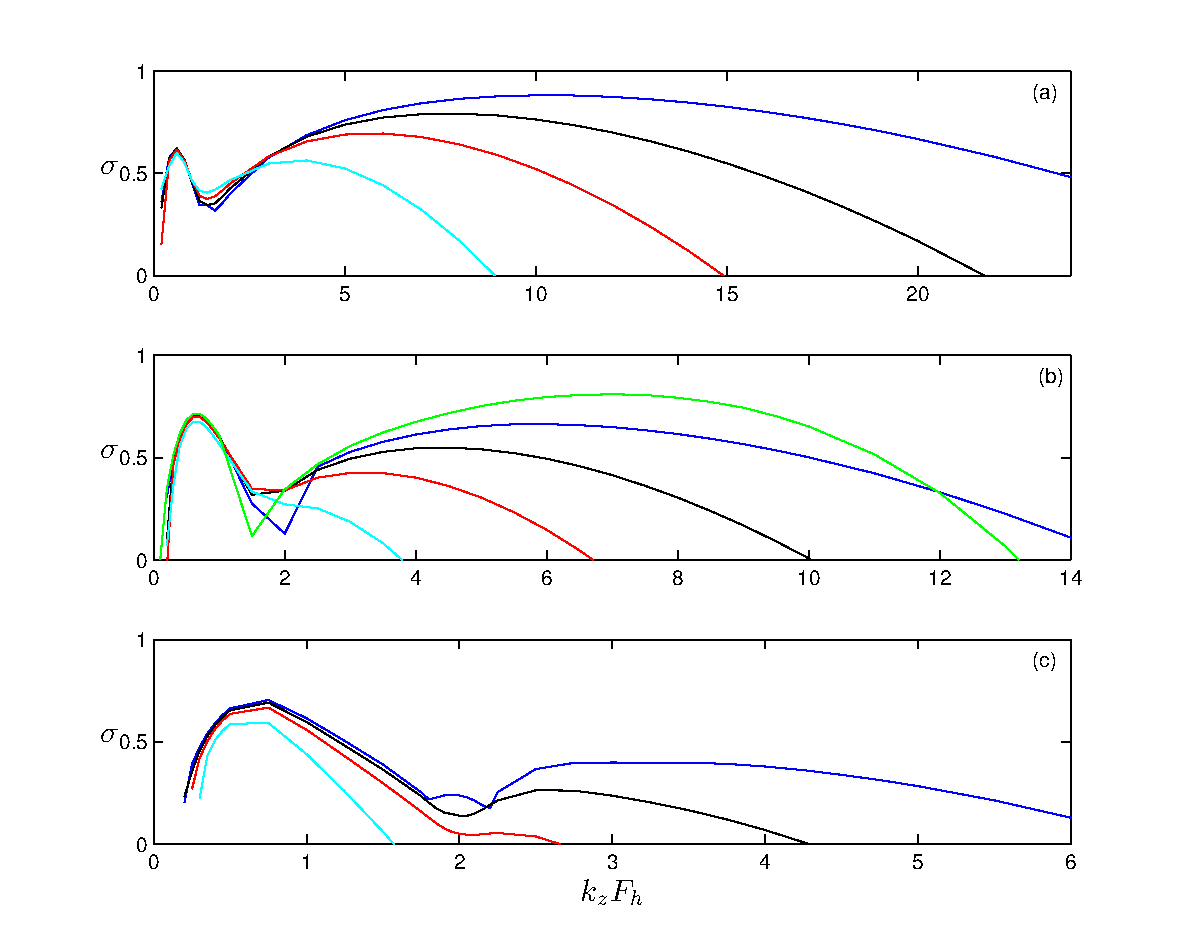
\includegraphics[width=\textwidth]{fixed_froude_varying_reynolds.eps}
%\caption{Growth rate $\sigma$ as a function of $k_{z}F_{h}$ for fixed $F_{h}=$(a) $0.2$, (b) $0.1$, (c) $0.05$ with Re$=2000$ (cyan), Re$=5000$ (red), Re$=10000$ (black), Re$=20000$ (blue). In panel (b) the green line is the hyperviscosity case with $Re=20000$.}
%\label{FixFhVaryRe}
%\end{center}
%\end{figure}
%\begin{figure}
%\begin{center}
%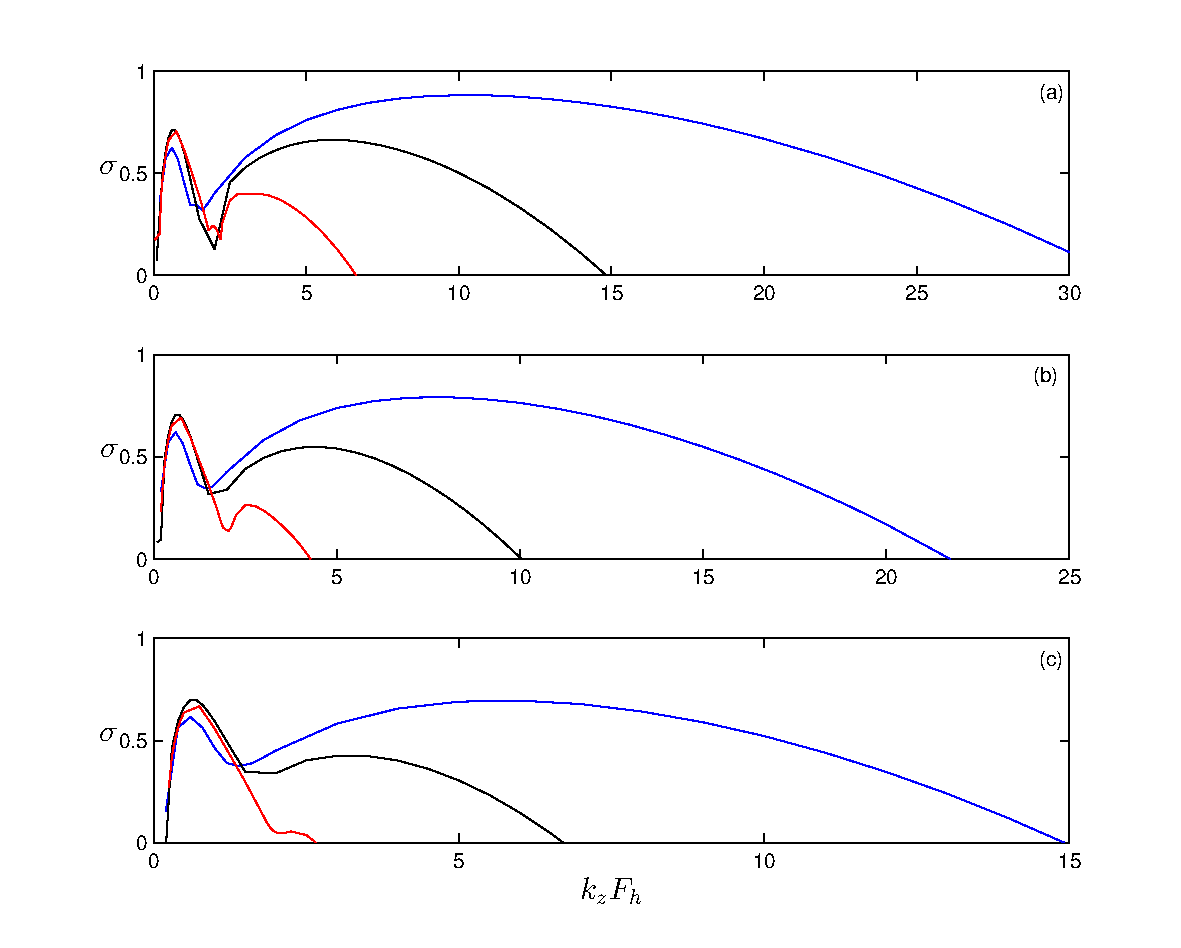
\includegraphics[width=\textwidth]{fixed_reynolds_varying_froude.eps}
%\caption{Growth rate $\sigma$ as a function of $k_{z}F_{h}$ for fixed $\text{Re}=(a) 20000, (b) 10000, (c) 5000$ with $F_{h}=0.05$ (red), $F_{h}=0.1$ (black), $F_{h}=0.2$ (blue).}
%\label{FixReVaryFh}
%\end{center}
%\end{figure}
The above analysis demonstrates that the short-wave growth-rate peak moves to larger $k_{z}F_{h}$ with increasing $F_{h}$ and increasing $Re$, but has a stronger dependence on Froude than Reynolds. Some of this joint dependence can be explained by examining the dependence on the buoyancy Reynolds number $Re_{b}=F_{h}^{2}Re$ \cite{riley2003,hebert2006,brethouwer2007}. In stratified turbulence, the buoyancy Reynolds number is analogous to the Reynolds number in the viscous term due to the vertical gradients \cite{brethouwer2007}. As $k_{z}$ increases, we move to smaller vertical scales where the vertical viscosity terms, controlled by the buoyancy Reynolds number, dominates, so it follows that the second peak may be governed by $Re_{b}$. In Fig.~\ref{Buoy} the location of the second peak from Fig.~\ref{FixFhVaryRe} is plotted as a function of the buoyancy Reynolds number. The peak location line is approximately linear and can be fitted with the curve $k_{z}F_{h}= Re_{b}^{2/5}$, which is plotted. This scaling implies that the vertical wavenumber, $k_{z}$, of the short-wave instability is approximately 
\begin{align}
k_{z} \sim F_{h}^{-1/5} Re^{2/5}\label{buoyscale}.
\end{align} 
The dependence of the growth rate on $k_{z}F_{h}$ appears to be similar in the cases with different $F_{h}$ and $Re$ but the same $Re_{b}$. Fig.~\ref{ReBuoy} demonstrates the similarity of the growth rate plotted against $k_{z}F_{h}$ for two cases with $Re_{b}=500$ and two cases with $Re_{b}=50$. For both cases, the locations of the zigzag and second peak line up quite well. The difference between the red and blue curves at the second peak is $4\%$ for $Re_{b}=200$ and $6\%$ for $Re_{b}=50$, a reasonable variation. 

% It is interesting to note that the red curve, corresponding to $Re=20000$ and $F_{h}=0.1$ (a), $F_{h}=0.05$ (b), is lower then the blue curve, corresponding to $Re=5000$ and $F_{h}=0.2$ (a), $F_{h}=0.1$ (b). This supports the observation, and is clear from the definition of the buoyancy Reynolds number, that the stratification may play a more important role in the instability than the viscosity.   

%\begin{figure}
%\begin{center}
%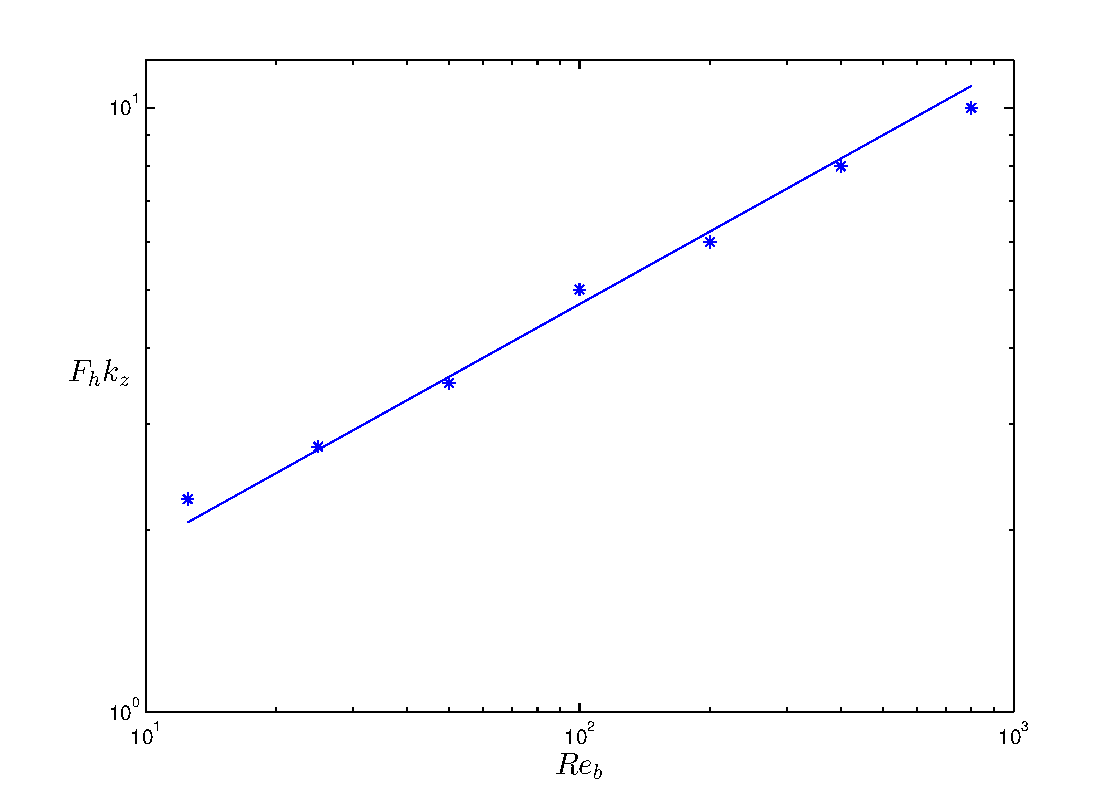
\includegraphics[scale=0.6]{second_peak_buoyancy.eps}
%\caption{The location of the second peak as a function of the buoyancy Reynolds number $Re_{b}$. $k_{z}F_{h}$ is taken from Fig.~\ref{FixFhVaryRe}. The straight line is $Re_{b}^{2/5}$.}
%\label{Buoy}
%\end{center}
%\end{figure}
%\begin{figure}
%\begin{center}
%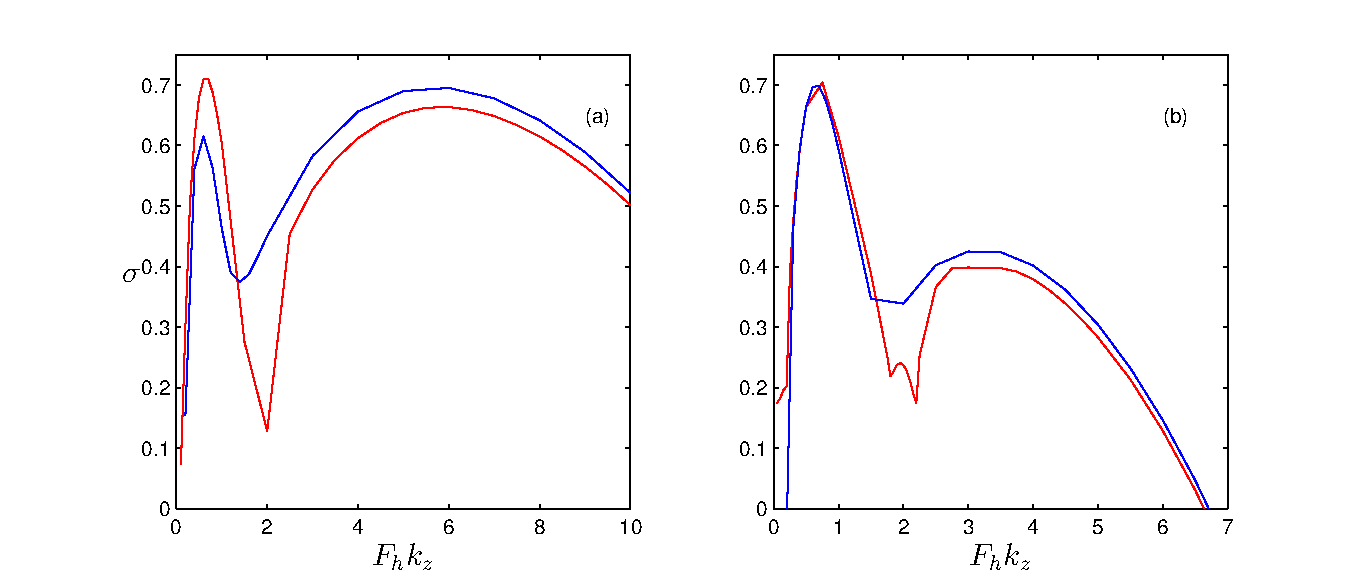
\includegraphics[width=\textwidth]{buoyancy_reynolds.eps}
%\caption{Growth rate $\sigma$ as a function of $F_{h}k_{z}$ for fixed $Re_{b}$. In (a), red is $Re=20000, F_{h}=0.1$ and blue is $Re=5000, F_{h}=0.2$, both corresponding to $Re_{b}=500$; in (b) red is $Re=20000, F_{h}=0.05$ and blue is $Re=5000, F_{h}=0.1$, both correpsonding to $Re_{b}=50$.}
%%\caption{Growth rate $\sigma$ as a function of $k_{z}$ for fixed $Re_{b}=(a) 200, (b) 50$. In (a) red corresponds to $Re=20000, F_{h}=0.1$ blue to $Re=5000, F_{h}=0.2$, in (b) red corresponds to $Re=20000, F_{h}=0.05$, blue $Re=5000, F_{h}=0.1$}
%\label{ReBuoy}
%\end{center}
%\end{figure}


In Fig.~\ref{FixFhVaryRe} (b) the green curve corresponds to a hyperviscosity run with $Re=20000$, which has $Re_{h}=2.8\times 10^{8}$. The motivation for using hyperviscosity is to capture higher-Reynolds number regime by restricting dissipation to only the largest wavenumbers. As the hyperviscosity run demonstrates, the zigzag peak is independent of Reynolds number and the existence of the peak would be expected at higher Reynolds numbers. For the second peak, we note that the growth rate  of the hyperviscosity run exceeds that of $Re=20000$ for $k_{z}F_{h}>3$ and reaches a maximum around $k_{z}F_{h}=7$. The maximum growth rate in the hyperviscosity case is around $25\%$ larger than the regular viscosity case with $Re=20000$. At $k_{z}F_{h}=12$ we see the hyperviscosity and non-hyperviscosity curves cross. This intersection corresponds to the horizontal wavenumber at which the hyperviscosity damping rate equals the regular viscous damping rate for $Re=20000$. For $k_{z}$ greater than this maximum, the hyperviscosity operator experiences greater damping than the regular viscosity, which can be seen by the sudden drop off of the growth rate. This simulation presents evidence that as $Re\rightarrow \infty$, the growth rate of the second peak will the same order as, or larger than, the growth rate of the zigzag instability. 

\subsection{Structure} 
%\begin{figure}
%\begin{center}
%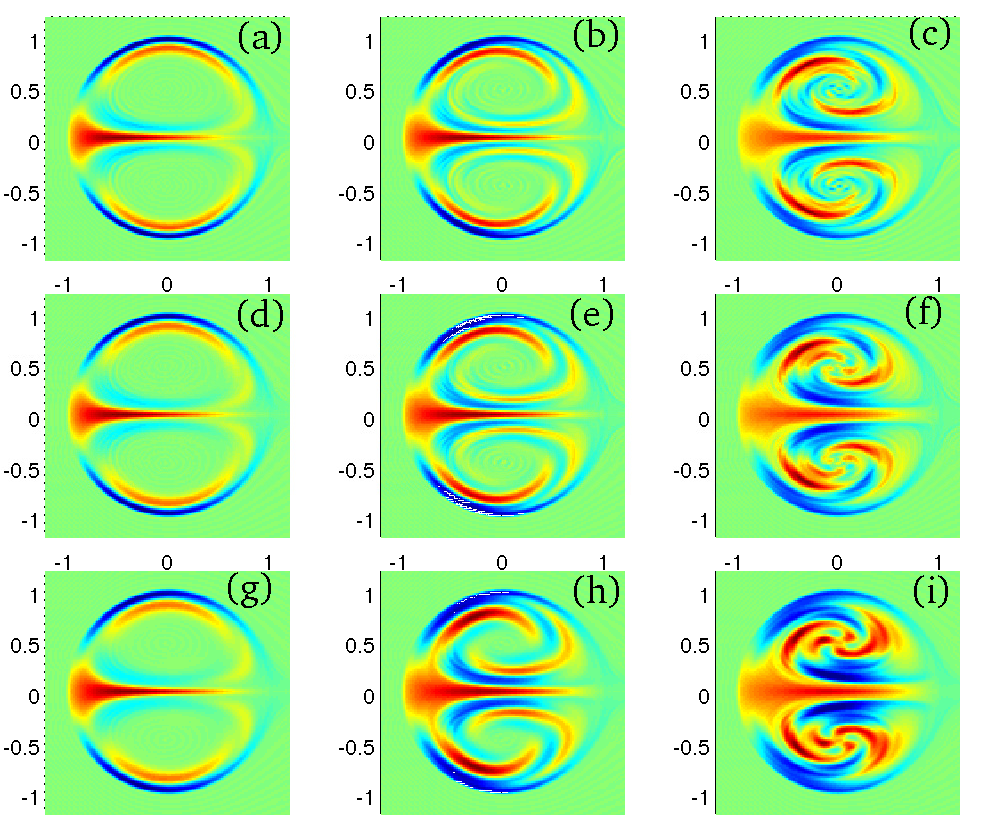
\includegraphics[width=\textwidth]{vorticity_second_peak.eps}
%%\caption{Perturbation vertical vorticity $\omega_{z}$ for $k_{z}$ at the second peak. $F_{h}=(a)(d)(g) 0.2 ,(b)(e)(h) 0.1, (c)(f)(i), 0.05, Re=(a)(b)(c) 20000, (d)(e)(f) 10000, (g)(h)(i) 5000$.}
%\caption{Perturbation vertical vorticity $\omega_{z}$ at second peak for $Re=20000\text{ (top) }, 10000 \text{ (middle) }, 5000 \text{ (bottom) }$; and $F_{h}=0.2 \text{ (left) }, 0.1 \text{ (middle) }, 0.05 \text{ (right) }$.}
%\label{secondpeak}
%\end{center}
%\end{figure}
Fig.~\ref{secondpeak} shows the spatial structure of the perturbation vertical vorticity at the second peak for different $Re$ and $F_{h}$. Qualitatively, we observe greater variation for different Froude numbers versus different Reynolds number as suggested above.  At the largest Froude number, the perturbation vorticity is organised in thin strips around and inside the dipole core between the two vortices. Panels (b),(e),(h) have $F_{h}=0.1$ and have a similar overall structure to the larger Froude number. Here, in the cores of the vortices, there is an emergence of a swirl-like pattern. At lower Reynolds number, the structure is spread out due to diffusion, while at higher Reynolds number, small-scale structure is beginning to emerge. This trend continues overall as we move to lower Froude numbers. 

Examining panels (g)-(i) (fixed $Re$ and decreasing $F_{h}$), the core of the dipoles has a twisting-like behaviour as the Froude number decreases. From this we can conclude that the instability structure of the second peak depends more on the Froude number than on the Reynolds number, which again reinforces the buoyancy Reynolds number scaling.  Indeed, if we consider the cases with $Re_{b}=50$ and $200$ as above, which correspond to Fig.~\ref{secondpeak} (b),(g) and (c),(h) respectively, we can see similar structure in the vorticity fields. Additionally, the anti-symmetric structure of the perturbation can be observed in the dominant eigenmodes in all cases, as found by Refs 17,26\nocite{bc1999,bc2000c}.

% The vorticity being very thin in the centre is consistent with the results of \cite{pierrehumbert1986} which examined unstratified inviscid vortices at small vertical scales which also demonstrated this behaviour. 
%\begin{figure}
%\begin{center}
%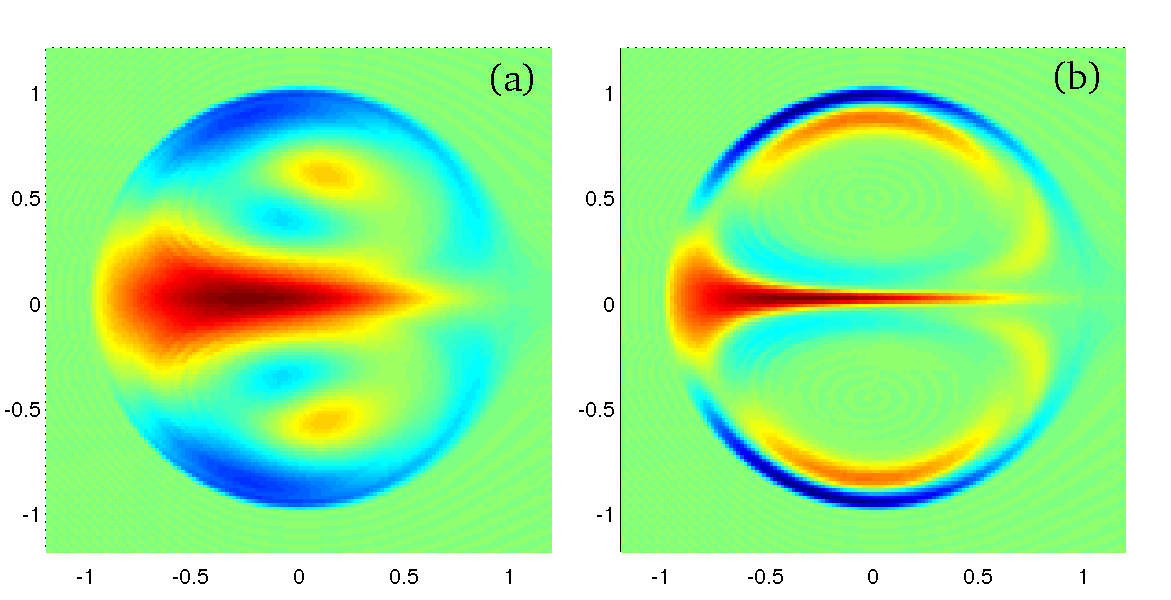
\includegraphics[scale=0.5]{second_peak_vs_zigzag.eps}
%\caption{Perturbed vertical vorticity $\omega_{z}$ at (a) the zigzag peak (b) the second peak for $Re=5000, F_{h}=0.2$}
%\label{zigzagcomparison}
%\end{center}
%\end{figure}

Fig.~\ref{zigzagcomparison} shows the perturbation structure for the zigzag peak (a) and the short-wave peak (b) for the case of $Re=5000,F_{h}=0.2$. This case was chosen because the growth rates of the two wavenumbers is roughly the same (see Fig~\ref{FixFhVaryRe} a). The zigzag instability exhibits a quadropole vorticity structure as discussed in Ref 17\nocite{bc2000c}, which corresponds to a bend and a twist of the basic state dipole. The short-wave instability shares some common overall structure with the zigzag instability. Both have a line of vorticity centred in between two Lamb-Chaplygin vortices and have a ring of vorticity negative vorticity around the outer edges of the dipoles. Additionally, the number of local maximum and minimum remains the same. However, in the short-wave instability, these bands of vorticity have been squeezed into thinner strips and are much more localised along the outer edges of the vortices. In the cores of the dipoles, there is almost no structure and we do not see a quadropole moment. The full vorticity field of the short-wave instability has a much more dominant twist then the zigzag instability and the bending of the dipole is reduced. As the stratification is increased, this behaviour continues but there is a significant emergence of structure within the cores of the vortices, as observed in Fig~\ref{secondpeak}.


\subsection{Subdominant modes?} 
The above analysis only provides the leading eigenvalue. Discuss subdominant mode ideas. Krylov method + matlab method.
\section{Dimensional Analysis}
That will go here. 


\section{Conclusion}



%-------------------------------------------------------------------------------
%
%   NONLINEAR THEORY 
%
%-------------------------------------------------------------------------------
%%%%%%%%%%%%%%%%%%%%%%%%%%%%%%%%%%%%%%%%%%%%%%%%%%%%%%%%%%%%%%%%%%%%%%%%%%%%%%%%%%%%%%%%%%%%%%%%%%%%
% NONLINEAR THEORY 
%
% 
%%%%%%%%%%%%%%%%%%%%%%%%%%%%%%%%%%%%%%%%%%%%%%%%%%%%%%%%%%%%%%%%%%%%%%%%%%%%%%%%%%%%%%%%%%%%%%%%%%%%
\chapter{Nonlinear theory}

\section{Introduction}
In the previous chapter, we investigated the linear stability of the Lamb-Chaplygin dipole and we showed that the short-wave instability can have growth rates that are comparable to those of the zigzag instability. An important question is if both of these instabilities exist, which will dominate in the transition to turbulence? In the atmosphere and ocean, a wide range of length scales are excited, so it is expected that both the zigzag instability and the short-wave instability will be excited in nature. Understanding the evolution of these two instabilities and what role they play in the transition to turbulence is important to correctly understand the mechanisms at play in the transition to stratified turbulence. Unfortunately, as alluded to in Chapter 2, linear stability analysis can only take us so far. 

In this chapter we evolve the full nonlinear Boussinesq equations to determine how the short-wave instability evolves and what role it plays in the transition to turbulence. The importance of the zigzag instability in the breakdown and transition to turbulence has been well studied \cite{augier2012,waitesmol2008,augierbillant2011,delonclebc2008} and none of these studies have mentioned short-wavelength instabilities. In this chapter we investigate the role of the short-wave instability in the transition to turbulence. Through nonlinear simulations, we will demonstrate that the saturation level of the short-wave instability is relatively small and depends upon the aspect ratio $\delta=L_{v}/L_{h}$. Thus, for many geophysical flows, where $\delta\ll 1$, the short-wave instability does not affect the overall breakdown and transition to turbulence. 

\section{Set-up} 
To investigate the nonlinear evolution, we use a code developed by Waite (and others? first paper to use is..?). The code implements the spectral method technique discussed in Chapter 3 to solve the nonlinear Boussinesq equations. Unlike in linear stability analysis, nonlinear analysis of the Boussinesq equations is much more complicated as particular attention must be taken to ensure proper resolution of the small scales. Although we are not doing a full dynamical numerical simulation (DNS), where we would be resolving everything, the breakdown of the zigzag instability exhibits small scale turbulence which suggests that we might observe a similar result for the short-wave instability. Thus we need to choose grid sizes that approximately resolve the smallest scales, known as the Kolmogorov scale. 

The Kolmogorov scale is given by \cite{lesieur}
\begin{align}
\eta = \left(\frac{\nu^{3}}{\epsilon}\right)^{3},
\end{align}
where $\epsilon$ is the kinetic energy dissipation rate, which is commonly approximated as \cite{lindborg2006}
\begin{align}
\epsilon \sim \frac{U^{3}}{R} ,
\end{align}
where $U,R$ are the characteristic velocity and length respectively. Rewriting the Kolmogorov scale $\eta$ in terms of the Reynolds number by multiplying by the characteristic length $R$ we obtain
\begin{align}
\frac{\eta}{R} = \frac{1}{\Re^{3/4}}.
\end{align}
As discussed previously, stratified flow has two distinct directions, the horizontal and vertical and thus for our simulations, the code sets the horizontal and vertical resolutions independently, which we denote by $\Delta x$ and $\Delta z$. We want to choose the number of grid points to be such that $\Delta x \approx \Delta z \approx \eta/R$.

To focus specifically on the short-wave instability, we choose the vertical scale to be that of the short-wave instability. To illustrate, consider $Re=2000, F_{h}=0.2$ where the short-wave instability peaks at $k_{z}=20$. Here the vertical scale is 
\begin{align}
L_{v} = \frac{2\pi}{k_{z}} = \frac{2\pi}{20}.
\end{align}
Note that this vertical scale also sets the scaling for the vertical wavenumbers in the full nonlinear simulation. From our linear results, we again take $L=9$. Due to the set-up of the code, the number of grid points in every direction has to be a power of $2$. Thus let us a priori consider the number of horizontal grid points to be $N=1024$. We have that the horizontal resolution is
\begin{align}
\Delta x = \frac{L}{N} = \frac{9}{1024}\approx 0.00878,\qquad \frac{\eta}{R}\sim \frac{1}{Re^{3/4}}=0.003343,
\end{align}
and we approximately have that $\Delta x \sim \eta/R$. Even though this may be cause for concern based on our definition of the Kolmogorov scale, DNS with $L=9$ has suggested that this resolution is sufficient (cite). If choose $N=32$ grid points in the vertical, we find that $\Delta z \approx 0.00982$ which is very similar to $\Delta x$. For our timestep we choose $\Delta = 5.0\times 10^{-4}$. Each run was initialised with a random density sinusoidal perturbation with $\epsilon=0.01$. 


\section{Results}
As mentioned in the introduction, previous investigations into the transition of turbulence have focused only on the zigzag instability. In all these simulations, it is clear that the dominant instability is the zigzag instability. For example, in Waite and Smolarkiewicz \cite{waitesmol2008}, the growth rates of the zigzag instability agree with the linear theory. It is possible that these simulations were not resolving the small scales, although this does not seem likely based on the parameters given. This is because the length scale of the short-wave instability is about an order of magnitude or so smaller than that of the zigzag instability. Since these simulations were intended to study the transition to turbulence, they would be resolving, or close to resolving, the Kolmogorov scale, which is much smaller than the short-wave instability. Hence it is unlikely a resolution issue. Instead, it could be the case that the short-wave instability is present but saturates out and does not contribute significantly to the transition to turbulence. We explore this option here. 

Consider the following scaling argument and results due to Ngan, et al.\cite{ngan2005}. They were interested in three-dimensionalisation of a two-dimensional flow, specifically the case of quasi-two dimensional turbulence, which is an in-between case between 2D turbulence and 3D turbulence. They considered this as they were interested in geophysical flows which exhibit small aspect ratios, $\delta=0.01-0.1$ \cite{ngan2005}. As we have seen, stratified turbulence tends to have a small aspect ratio and, as discussed in Chapter 2, exhibits characteristics of quasi-geophysical flow which shares characteristics with a two-dimesional flow being three-dimensionalised. However, it is important to note that Ngan et al.\cite{ngan2005} did not consider stratification and they were only focusing on the unstratified case of turbulence with small aspect ratios. 

To investigate this three-dimensionalisation, in their numerical experiments they took fully developed 2D turbulence and subjected it to a 3D perturbation. They then measured the saturation level of this 3D perturbation. The saturation level is defined to be
\begin{align}
\text{saturation} = \frac{u}{U}\bigg|_{t=sat}, \label{ngan_scale}
\end{align}
where the ratio between the 3D velocity $u$ and the 2D velocity $U$ are evaluated at the saturation time. The saturation time is the time at which the time series of the 3D velocity levels off or saturates. They found, numerically, that this saturation level depended linearly on the aspect ratio $\delta$, up to a certain aspect ratio, $\delta=0.5$. Beyond $\delta=0.5$ the numerical simulations could no longer be considered quasi-two dimensional. 

To explain this result, Ngan et al. considered a simple scaling argument \cite{ngan2004,ngan2005}. Initially the time scales of the 2D base flow is long compared to that of the 3D perturbation flow. However once the 3D perturbation settles down and saturates, its timescale becomes similar to that of the 2D flow.  Consider the following timescales for these flows \cite{ngan2005} as
\begin{align}
T_{2D} = \frac{U}{L},\qquad T_{3D} =\frac{u}{H}
\end{align}
where $U$ is the characteristic velocity of the 2D flow at saturation and $u$ is the characteristic velocity of the 3D flow at saturation. At saturation $T_{2D}\sim T_{3D}$ and thus we have that 
\begin{align}
\frac{U}{L}\sim\frac{u}{H} \Rightarrow \frac{u}{U} \sim \frac{H}{L} = \delta,
\end{align}
which is the result they confirmed numerically. 

Motivated by this result, we consider the saturation levels of the short-wave instability for $Re=2000,5000$ and $F_{h}=0.2$. These two cases were chosen as they both had short-wave instability growth rates similar to that of the zigzag peak. Higher $Re$ could not be explored due to resolution issues, as alluded to in the previous section. We differ from Ngan et al.\cite{ngan2005} in that we instead consider the energy instead of the velocity.\begin{align}
\text{saturation} = \frac{E_{2D}}{E_{3D}}\bigg|_{t=sat}.
\end{align}
Additionally, unlike Ngan et al.\cite{ngan2005} we also have potential energy.  

To compute the saturation level, the code allows for two possibilities. The first is to compute the kinetic and potential energy directly from the definition, as discussed in Chapter 3. The other is to compute the 2D and 3D energy directly from the vertical spectrum. 

In the first case, we compute the kinetic and potential energies and associate the 2D flow with the kinetic energy and the 3D perturbation with the potential energy. This is justifiable by realising that the basic state, the Lamb-Chaplygin dipole, is initially kinetic energy only and thus the potential energy is coming strictly from the 3D perturbation. 

The other method is to determine the 2D and 3D energy directly summing the vertical spectrum. In our simulations, the vertical spectrum had wavenumbers $k_{z}=0,1,\ldots,11$. Recall that here $k_{z}$ has been non-dimensionalised with the short-wave instability and thus $k_{z}=1$ corresponds to the wavelength of the short-wave instability. $k_{z}=0$ corresponds to the 2D dimensional energy and the sum of the remaining wavenumbers corresponds to the 3D energy. 

Both methods were used to compute the saturation level and it was found that the results using the kinetic and potential energy were better than directly computing the 2D and 3D energy from the vertical spectrum. Fig.~\ref{sat_energy} demonstrates the results for $Re=5000, F_{h}=0.2, k_{z}=40$. As can be observed in the Figure, the kinetic (2D) energy from both methods are very similar and nearly indistinguishable. The big difference is for the potential (3D) energy. The spectrum method (dashed-blue) is more jagged (?) and the saturation level is less well defined. The direct computation of the energy (black) is smoother, although still has bumps, but the saturation level is approximately constant. For this reason, we choose to use the direct computation of the energy. Despite the differences, both curves have the same saturation time, roughly $T=20$. 
\begin{figure}
\begin{center}
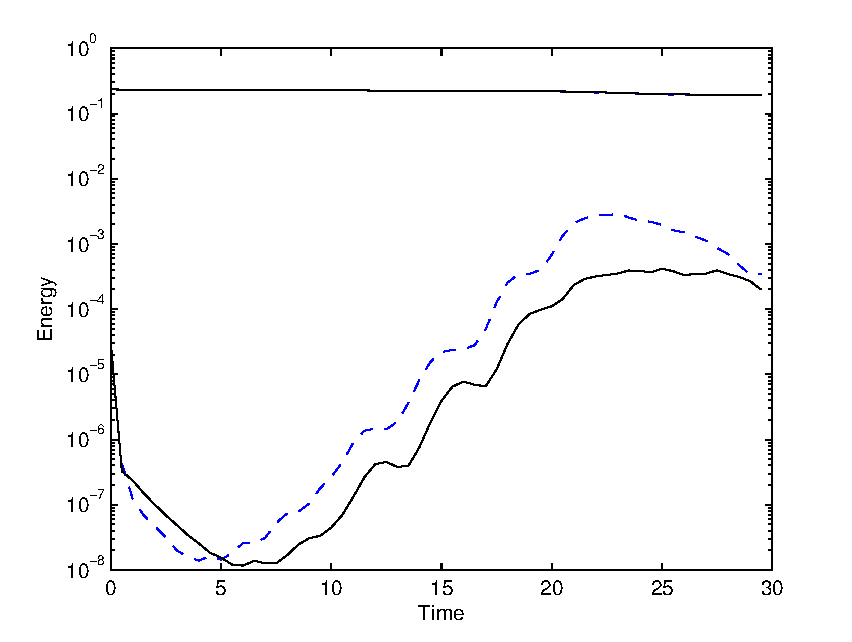
\includegraphics[width=\textwidth]{sat_eg_re5000_fh02}
\caption{Time series demonstrating the two ways of computing the energy for $Re=5000, F_{h}=0.2, k_{z}=40$. The dashed blue curves correspond to computing the energy through the vertical spectrum and the solid black curves correspond to the computing the energy directly from the fields. The top line corresponds to kinetic (2D) energy and the bottom lines correspond to potential (3D) energy.}
\label{sat_energy}
\end{center}
\end{figure}

However computing the energy from the vertical spectrum does allow for the contributions due to each wavenumber. Fig.~\ref{other_kz} demonstrates this for previous parameters. Here we can explicitly see which wavenumbers are contributing to the total 3D energy. For almost the entire simulation, the $k_{z}=1$ wavenumber dominates, as the total sum of the wavenumbers is obscured by $k_{z}=1$. However at around the saturation time $T=20$, $k_{z}=2$ appears to be contributing as the total 3D energy is a little above $k_{z}=1$. This lasts for about $5$ time units before diffusion begins to rapidly diffuse out the smaller scales, which is especially evident in the highest wavenumbers. 
\begin{figure}
\begin{center}
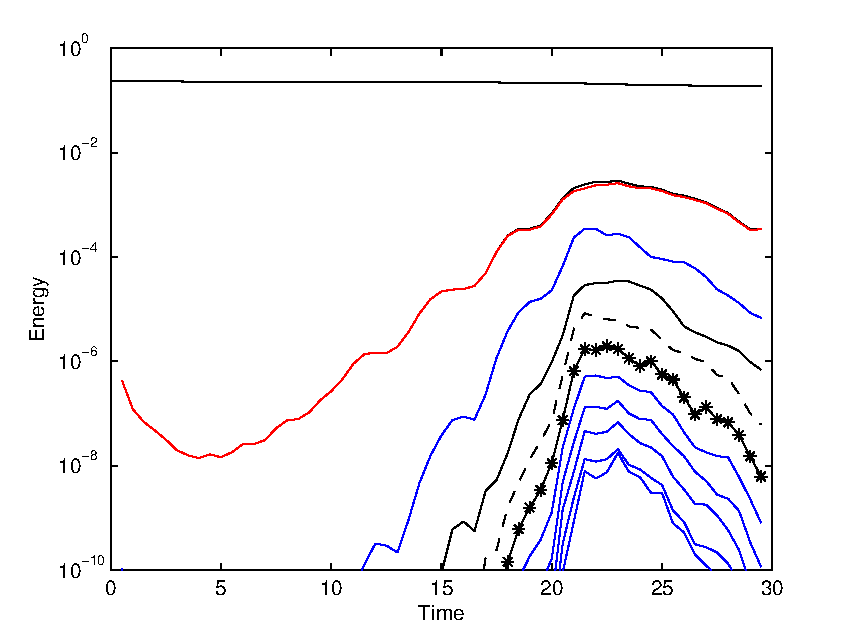
\includegraphics[width=\textwidth]{other_kz}
\caption{Time series for the energy computing from the vertical spectrum $Re=5000, F_{h}=0.2, k_{z}=40$ for different vertical wavenumbers. The top black curve corresponds to $k_{z}=0$ and is the kinetic energy. In order from top to bottom: red curve is $k_{z}=1$, blue curve is $k_{z}=2$, black curve is $k_{z}=3$, dashed black is $k_{z}=4$, star is $k_{z}=5$, and so on. The black curve that is obscured by $k_{z}=1$ is the sum of all the nonzero vertical wavenumbers.}
\label{other_kz}
\end{center}
\end{figure}

To determine the saturation level as a function of $\delta$, we investigated a range of $k_{z}$ around the short-wave instabilities for $Re=2000,5000, F_{h}=0.2$. Fig.~\ref{re2000sat} is the case of $Re=2000$. The saturation levels follow an increasing trend which agrees with Ngan et al.\cite{ngan2005}: as the aspect ratio is increased, the saturation level increases. Using a least-squares fit we find that the best fit curve is $3.02$ and have plotted a reference curve of slope $3$. Fig.~\ref{re5000sat} is the case of $Re=5000$. Again, the trend of saturation level with increasing aspect ratio is observed here. Using a least-squares fit we find that the best fit curve is $3.16$ and a reference curve of slope $3$ is plotted. At this higher Reynolds number, it was observed that although the saturation was clear, the actual time to choose to evaluate the saturation ratio was not well defined. In Fig.~\ref{sat_energy} although the saturation level here is fairly flat, there is still a bit of variation in the saturation level. In some cases this variation was more pronounced so defining where to evaluate the saturation ratio was not well defined. For consistency, the first maximum after $T=20$ time units was chosen. 

\begin{figure}
\begin{center}
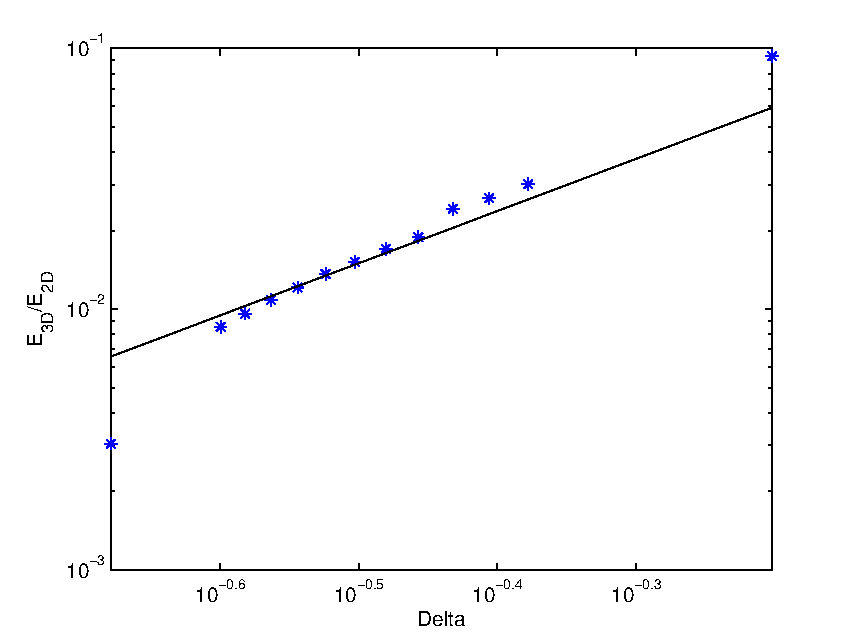
\includegraphics[width=\textwidth]{re2000_fh02_saturations} 
\caption{Saturation levels for a range of aspect ratios $\delta$ for $Re=2000$ and $F_{h}=0.2$. The curve has slope $3$.}
\label{re2000sat}
\end{center}
\end{figure}
\begin{figure}
\begin{center}
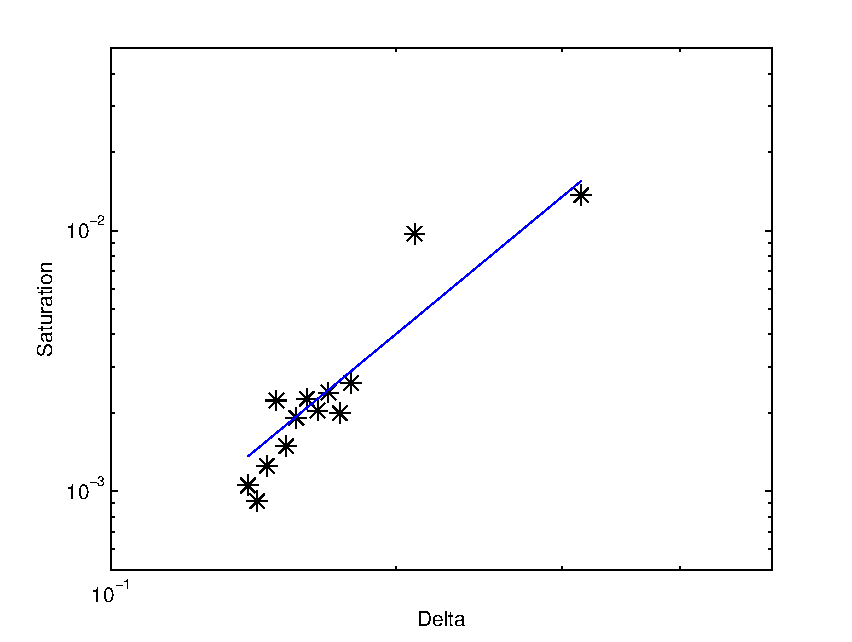
\includegraphics[width=\textwidth]{re5000_fh02_saturation_levels} 
\caption{Saturation levels for a range of aspect ratios $\delta$ for $Re=5000$ and $F_{h}=0.2$. The curve has slope $3$. }
\label{re5000sat}
\end{center}
\end{figure} 
From these two curves it suggests that the saturation level of the short-wave instability is given by
\begin{align}
\frac{E_{2D}}{E_{3D}}\bigg|_{t=sat} \sim \delta^{3},
\end{align}
which suggests that as the aspect ratio decreases, the saturation level decreases. From the linear theory, the short-wave instability was found to scale as $k_{z}\sim F_{h}^{-1/5}Re^{2/5}$ or $k_{z}'\sim F_{h}^{-1/5}Re^{2/5}/R$ in dimensional units. Then the aspect ratio scales as $\delta \sim F_{h}^{1/5}Re^{-2/5}$ and hence the saturation level is 
\begin{align}
\frac{E_{2D}}{E_{3D}}\bigg|_{t=sat} \sim (2\pi)^{3}F_{h}^{3/5}Re^{-6/5}.
\end{align}
Plugging in $Re=5000$ and $F_{h}=0.2$ yields a ratio on the order of $10^{-3}$ which agrees with Fig.~\ref{sat_energy}. For $F_{h}\ll 1$ and $Re\gg 1$ this ratio is $\ll 1$. Thus given that the short-wave instability seems to saturate at a relatively low level, we should not expect the short-wave instability to play a significant role in the evolution of the Lamb-Chaplygin dipole's transition to turbulence. 

This scaling for the saturation level differs from that of Ngan et al.\cite{ngan2005}. If we square Eq. (\ref{ngan_scale}) we obtain 
\begin{align}
\frac{u^{2}}{U^{2}} =\frac{KE_{3D}}{KE_{2D}}\sim \delta^{2},
\end{align}
which suggests that the saturation level will square quadratically instead of cubically. It is clear that their simple dimensional argument breaks down when stratification occurs, but this is not too surprising since the origins of their argument \cite{ngan2004} is based on a ``pressureless" argument where 
\begin{align}
\frac{|\nabla_{h}p|}{|\bm{u}\nabla\bm{U}|}= \mathcal{O}(\delta^{2}).
\end{align}
Using our scaling from Chapter 4, we would find, with $\rho_{0}=1$ following \cite{ngan2004}
\begin{align}
\frac{|\nabla_{h}p|}{|\bm{u}\nabla\bm{U}|}= \mathcal{O}(\delta^{-1}),
\end{align}
which is very different. Thus, we cannot use their scaling argument here. However, the similarities in results does suggest that such a dimensional argument might be possible.

Fig.~\ref{full_structure} is the vertical vorticity at three times, $T=15,20,25$. Recall that $T=20$ is the saturation time. Just before, $T=15$, the saturation the structure of the dipole does not exhibit any small-scale features. However at $T=20$, the saturation time, the dipole exhibits many small-scale features but by $T=25$ they have potentially been diffused out and the structure of the dipole has similar structure to itself before saturation, albeit with the two cores of the dipole more homogeneous in vorticity. The structure suggests that the saturation time is important as the dipole is undergoing some sort of transition, but as we saw, this transition is short lived as $5$ time units later, small-scale behaviour has potentially diffused out and there is no suggestion that the system will transition to turbulence. Indeed, this result reaffirms that the gridspace is sufficient enough to resolve the nonlinear evolution. Since this plot does not exhibit any features of turbulence, needing to resolve the Kolmogorov scale is not required. 
\begin{figure}
\begin{center}
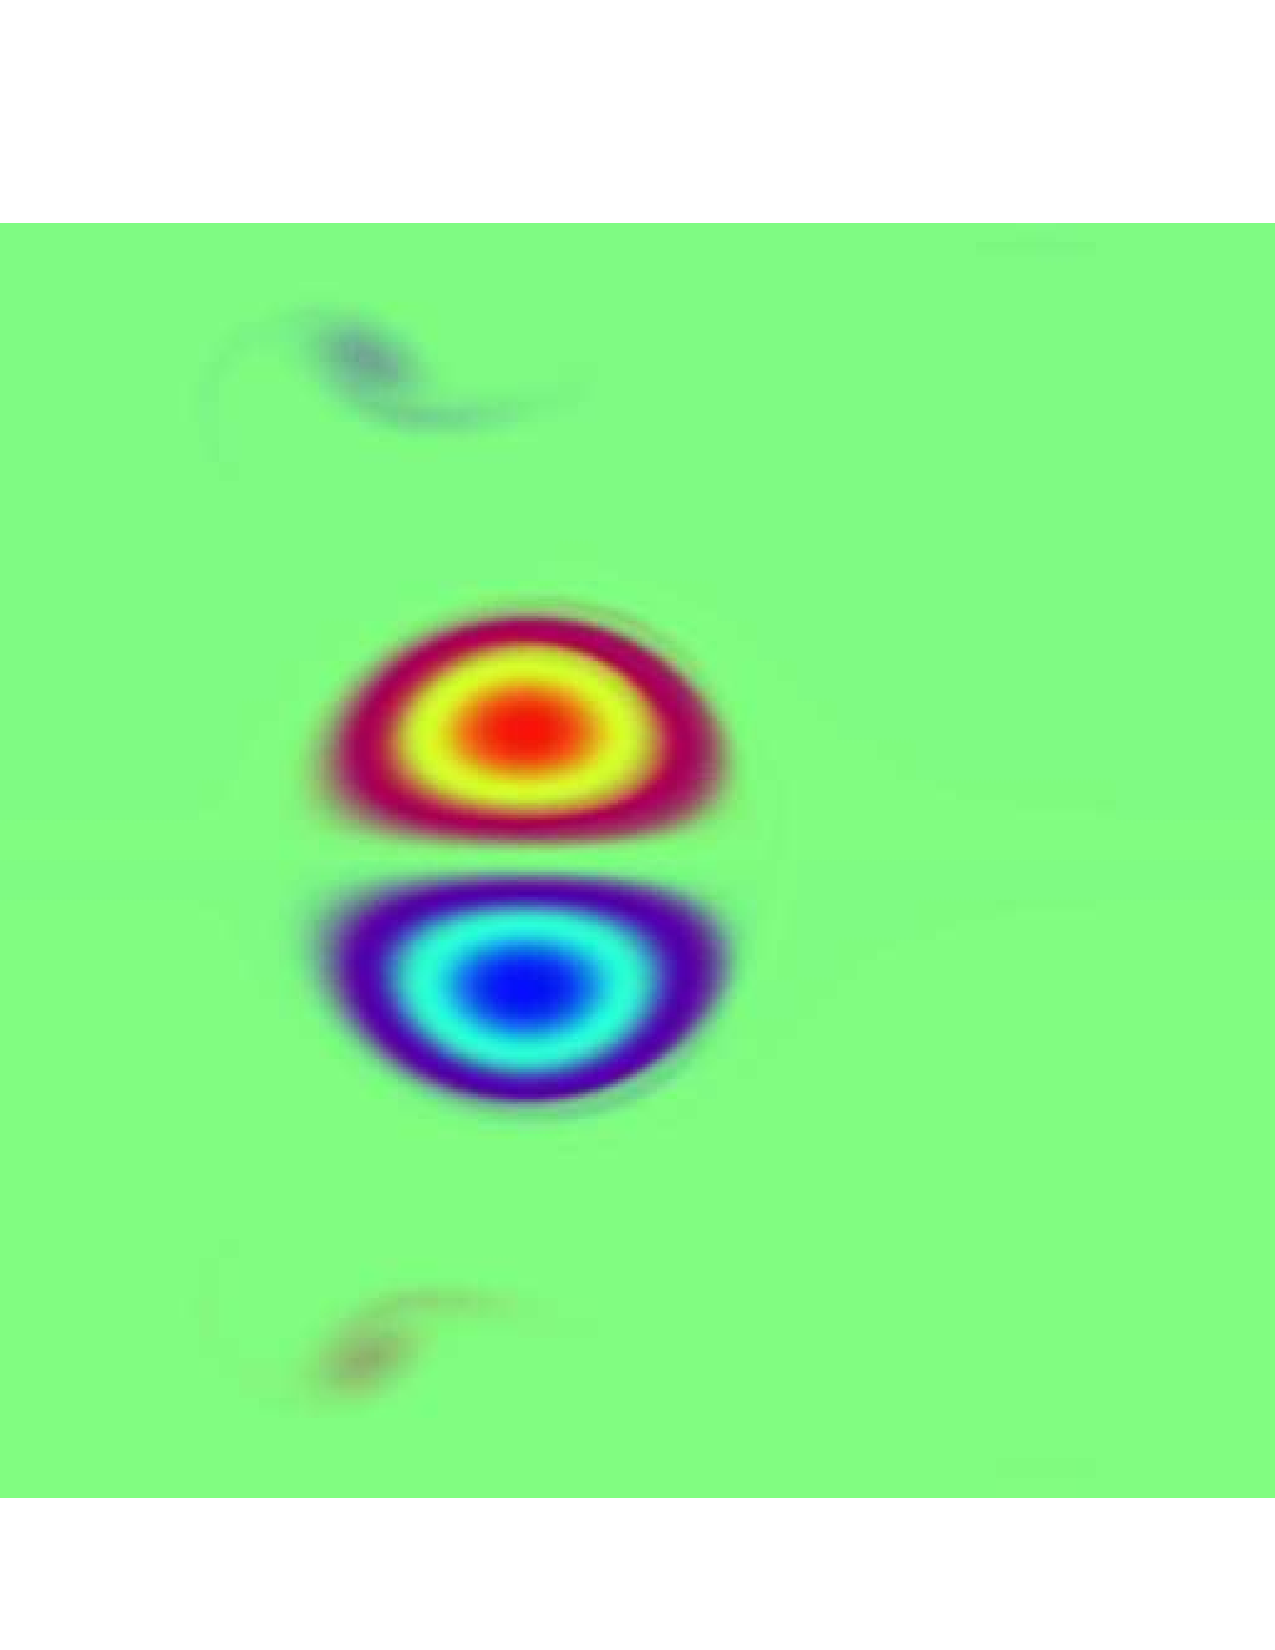
\includegraphics[width=0.4\textwidth]{struc_3}
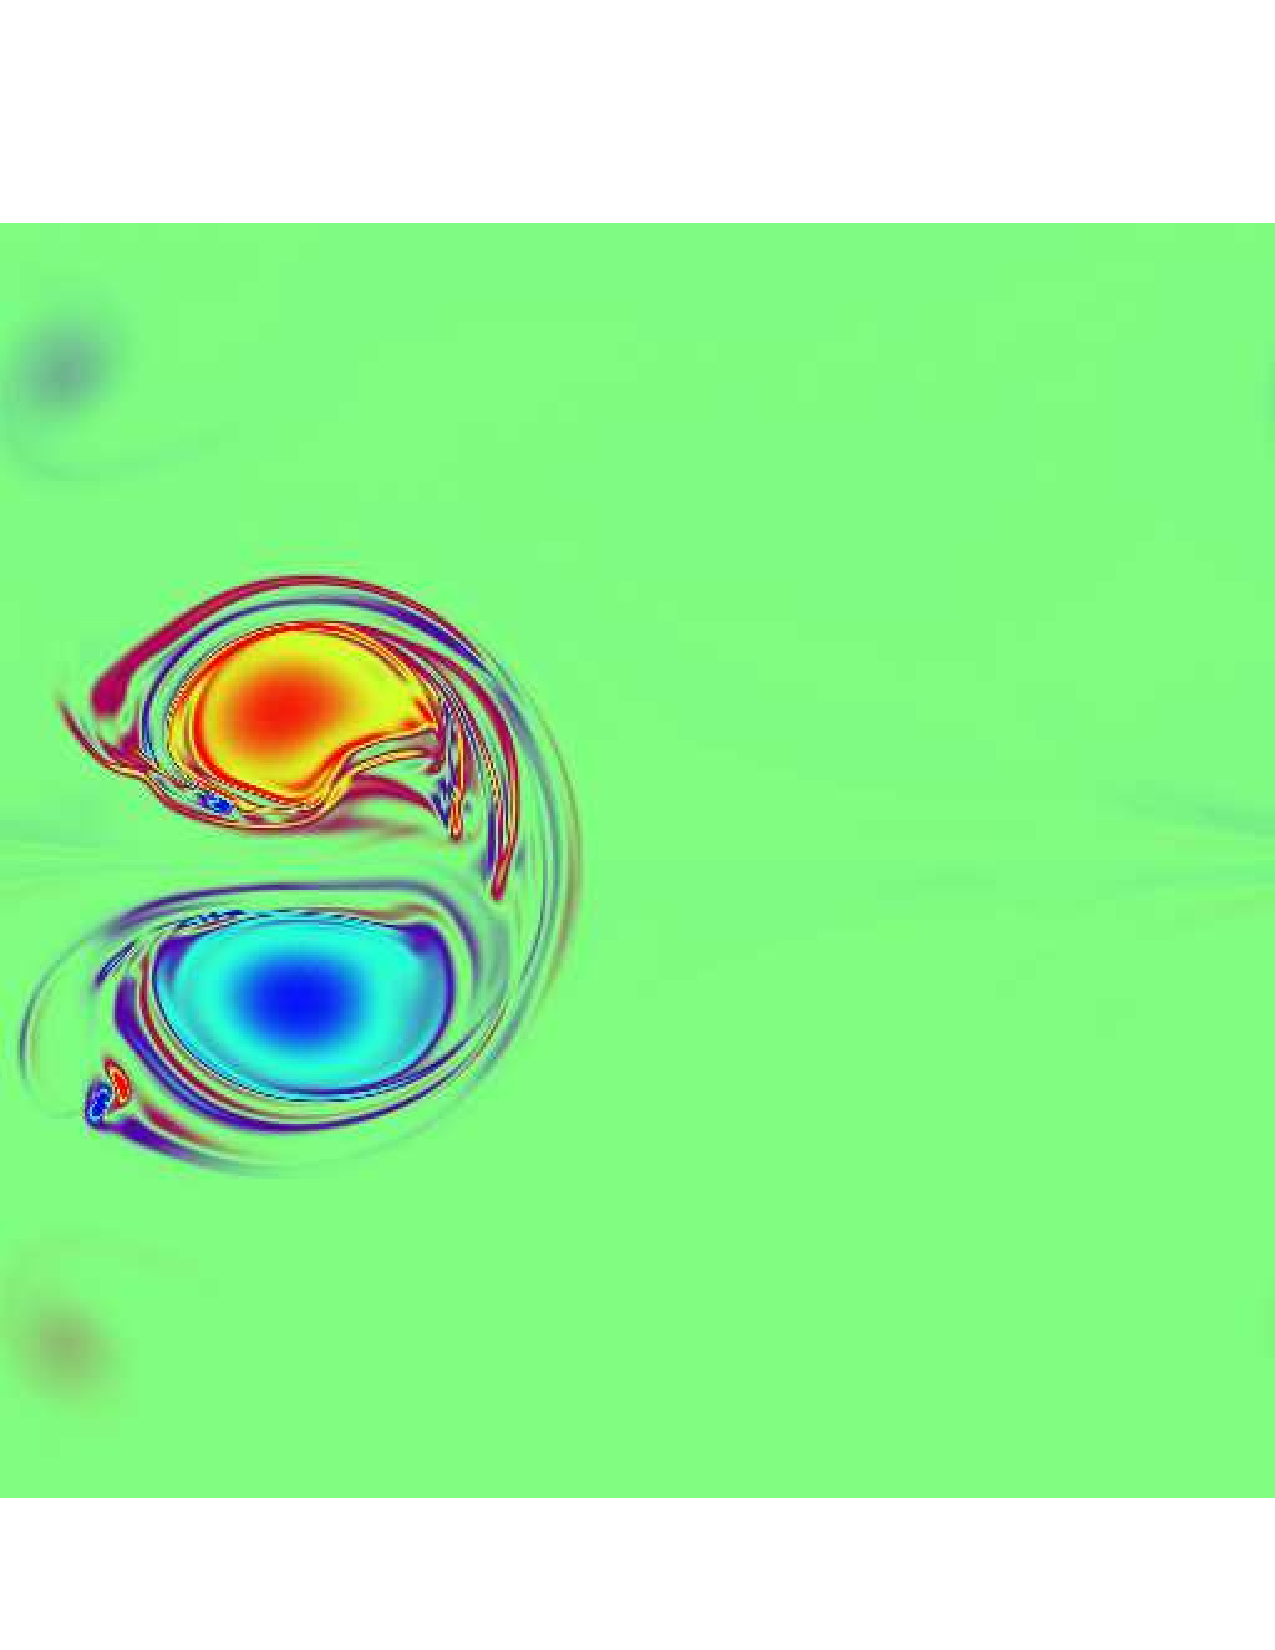
\includegraphics[width=0.4\textwidth]{struc_4}
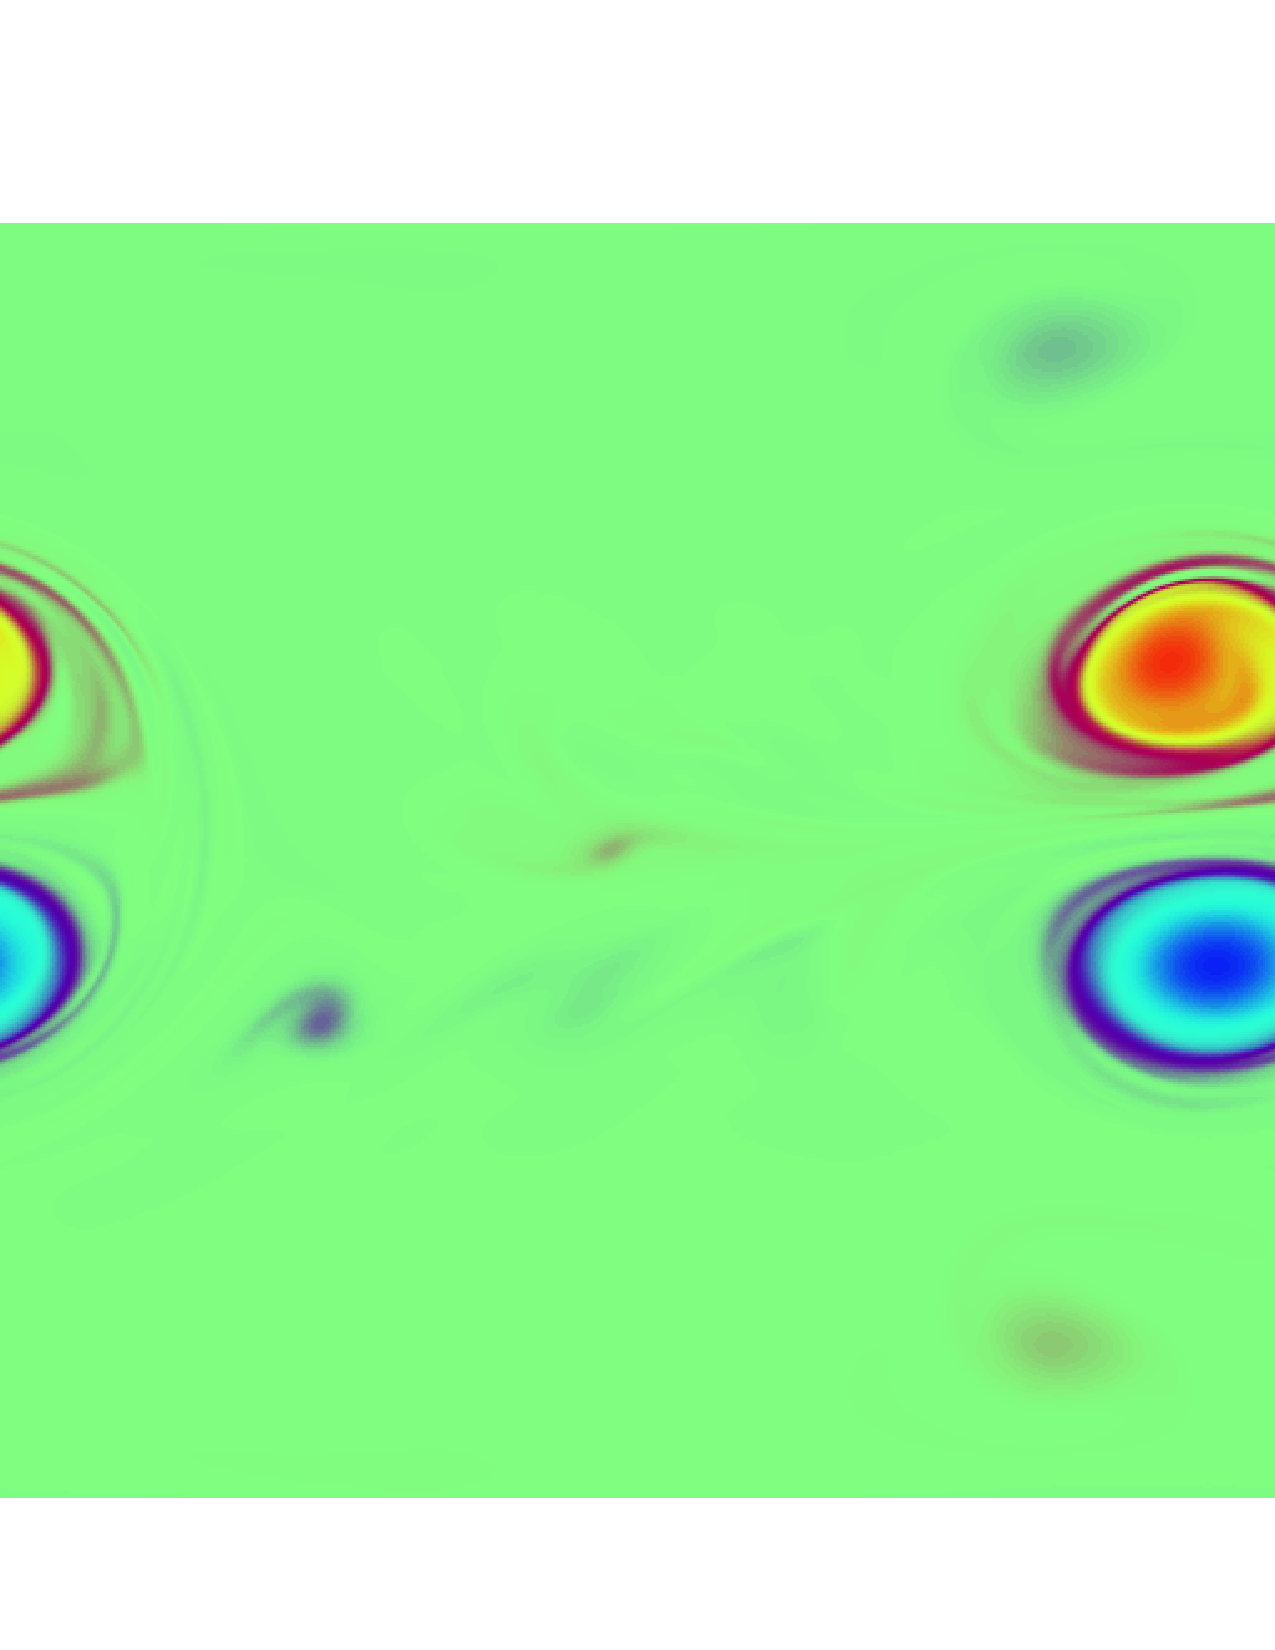
\includegraphics[width=0.4\textwidth]{struc_5}
\caption{Evolution of the vertical vorticity for $Re=5000, F_{h}=0.2, k_{z}=40$ for $T=15$ (top right), $T=20$ (top left), $T=25$ (bottom). Red corresponds to maximum vorticity and blue corresponds to minimum vorticity.}
\label{full_structure}
\end{center}
\end{figure}

We now examine the growth rate of the linear theory and that of the nonlinear theory. In comparing the linear theory with the nonlinear theory, there is a problem with what defines the linear regime of the nonlinear simulation. If we examine Fig.~\ref{sat_energy}, the growth of the potential energy between $T=5$ and $T=20$, it is very difficult to justify approximating this growth rate as linear. For most of the cases of $Re=5000$ and $F_{h}=0.2$, we were unable to determine a consistent way to determine the growth rate of the perturbation and thus we have not included the results for this simulation. Fig.~\ref{growth_rates_nonlinear} illustrates the results for the linear and nonlinear theories for $Re=2000$ and $F_{h}=0.2$. Here the nonlinear results are greater than those of the linear theory, however the curve still follows the linear theory curve. Again, the issue of the growth in the potential energy not being perfectly linear could contribute to this discrepancy of $8\%-40\%$. 

\begin{figure}
\begin{center}
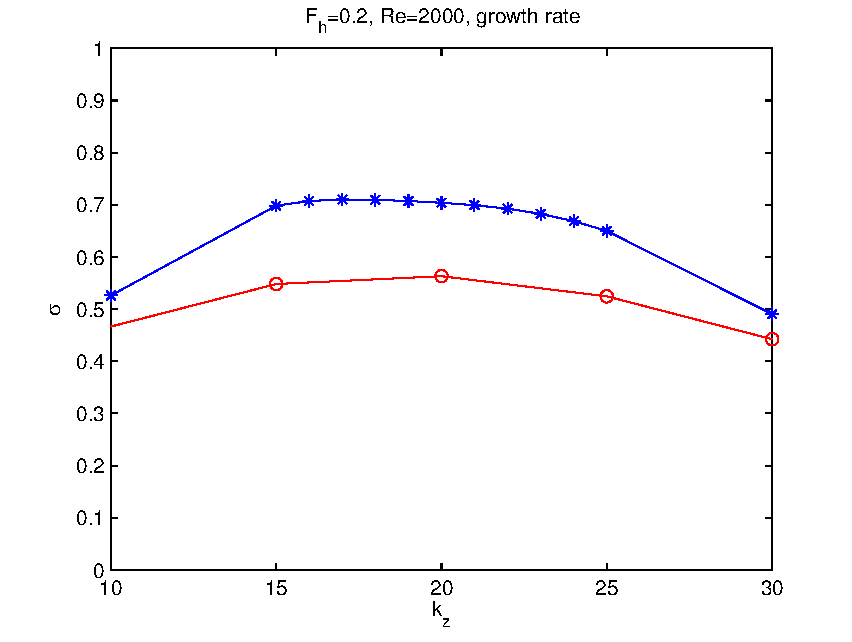
\includegraphics[width=\textwidth]{re2000_fh02_growth_rates} 
\caption{Growth rate for $Re=5000$ and $F_{h}=0.2$ with the linear results (red) and the nonlinear results (blue). Note we have not scaled by $F_{h}$ unlike the results in Chapter 3.}
\label{growth_rates_nonlinear}
\end{center}
\end{figure}

We conclude with a brief discussion of the consistency of the results. To ensure our results were consistent, we ran another simulation with $L=5$ and $N=64$ for the vertical wavenumber. This increase in the number of grid points in the vertical is to ensure that $\Delta x \sim \Delta z$ because decreasing $L$ decreases $\Delta x$ so $\Delta z$ must do so similarly. The results are plotted in Fig.~\ref{test_energy}. As can be observed, the overall amount of energy in the system is higher with $L=5$ because the domain is smaller and hence the dipole takes up a greater percentage of available grid points. Calculating the saturation level, here taken to be the maximum of the potential energy, yields a difference of $2\%$ between $L=5$ and $L=9$. In calculating the growth rate there is a difference of $8\%$. Thus if we increase the resolution, we will obtain similar results. Due to the way the code was set-up, using $L=5$ was not feasible to use as doubling the number of vertical grid points approximately doubled the simulation time. 
\begin{figure}
\begin{center}
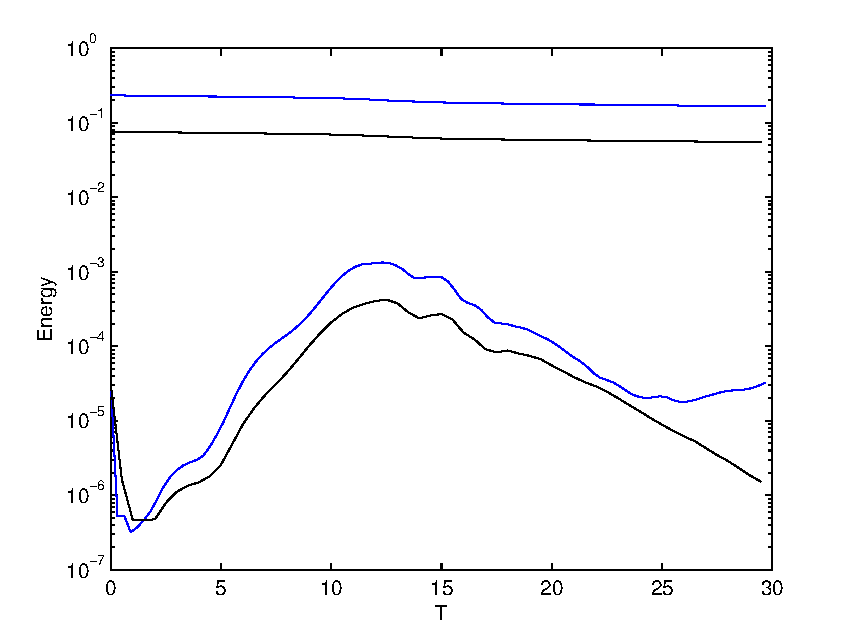
\includegraphics[width=\textwidth]{energy_test}
\caption{Time series of the potential energy (bottom curves) and kinetic energy (top curves) for $L=5$ (blue) and $L=9$ (black). Here $Re=2000, F_{h}=0.2,k_{z}=20$.}
\label{test_energy}
\end{center}
\end{figure}







%-------------------------------------------------------------------------------
%
%   CONCLUSIONS
%
%-------------------------------------------------------------------------------
\chapter{Conclusions}

In this thesis, we have investigated the linear stability of the Lamb-Chaplygin dipole for perturbations with small vertical scales. In particular, we have considered vertical scales from around the buoyancy scale $U/N$, where the zigzag instability occurs \cite{bc2000c,bc2001,waitebartello2004,waite2011}, down to the dissipation scale. We have discovered a short-wave instability that emerges at scales much smaller than the buoyancy scale. This instability can exhibit a growth rate that is comparable to, and possibly even greater than, that of the zigzag instability. Despite having a similar growth rate in some cases, the structure of the instability is qualitatively different that of the zigzag peak suggesting a different mechanism is governing the evolution.  We have discovered that the location of the peak depends upon a combination of the Reynolds and Froude numbers, specifically the buoyancy Reynolds number $Re_{b}$ which plays an important role in stratified fluids. The wavenumber of maximum growth rate for the short-wave instability is found to scale like $F_{h}k_{z}\sim Re_{b}^{2/5}$ for the range of $Re_{b}$ considered here. We expect this may change at even larger $Re_{b}$. By contrast, the maximum growth rate of the zigzag instability occurs for $F_{h}k_{z}\sim 1$ \cite{bc2000b}. As a result, these instabilities will be widely separated when $Re_{b}\gg 1$, as in the case of strongly stratified turbulence \cite{brethouwer2007}.

Despite the similar growth rates, we have discovered that these short-wave instabilities saturates at a level proportional to the cubed of the aspect ratio. For geophysical applications, $\delta$ is frequently $\ll 1$, which suggests that the short-wave instabilities do not contribute significantly to the breakdown of the Lamb-Chaplygin dipole to turbulence.

Some unanswered questions still remain and provide inspiration for future work. Structure-wise the short-wave instability is very different from that of the zigzag instability. As suggested by the sub-dominant mode analysis, there is likely a transition of leading eigenmodes between the zigzag and short-wave peaks. Furthermore, the nature of this transition is also interesting as it exhibits oscillations not observed in either the short-wave or zigzag instabilities. Briefly discussed were the waves behind the dipole, which resmeble a ship wave pattern with an angle that follows a simple scaling law. Investigations into waves behind vortices, especially those behind stratified vortices, has remained unexplored. Such flow might resemble flow over terrain which predicts a similar scaling law for the angle of those waves \cite{sharman1983ship}. Finally, it would be interesting to investigate the short-wave instability in other systems, specifically adding in the effects of rotation. Such investigations of buoyancy length effects have illustrated the zigzag instability, which demonstrates the universality of the result in other flow configurations. It is likely that such short-wave instabilities may be universal as well, but more work is required to resolve this question. 




\appendix

% Add a title page before the appendices and a line in the Table of Contents
\chapter*{APPENDICES}
\addcontentsline{toc}{chapter}{APPENDICES}
%======================================================================
\chapter[Spectral Example in Matlab]{Matlab Code for Solving Advection Equation}
\label{AppendixA}
% Tip 4: Example of how to get a shorter chapter title for the Table of Contents 
%====================================================================== 

The following code is the MATLAB code for evaluating the advection-diffusion equation with 2/3s deliasing
\begin{verbatim}
%construct the grid and basic parameters
N=128; dx=2*pi/N; x=dx*(1:N);t=0;dt=dx/10;tf=5;nsteps=ceil(tf/dt);
c=0.2+sin(x-1).^2;
%store the wavenumbers
kx=[0:N/2-1 0 -N/2+1:-1];
%define cut to cut out the highest Fourier modes
cut=ones(1,N); ksq=kx.*kx;
%cut out the Fourier co-efficients according to dealiasing 
%because of wavenumber ordering cut out (most negative wave numbers start
%at N/2) e.g. (2/3)*(N/2) : (N/2+(1/3)(N/2) for 2/3s
cut(ceil(dealias_coeff*N/2):(N/2+ceil((1-dealias_coeff)*N/2))+1)=0;
%initial condition
u=exp(-100*(x-1).^2);uhat=fft(u);
%do initial timestep using Euler
Fold=-fft(c.*real(ifft(1i*cut.*kx.*uhat)));
uhat=(uhat+dt*Fold); 

%do Adams Bashforth
for i=1:nsteps
    F=-fft(c.*real(ifft(1i*cut.*kx.*uhat)));
    uhat=uhat+1.5*dt*F-0.5*dt*Fold;
    Fold=F;
end
\end{verbatim}
In the above code the line \texttt{ifft(1i*cut.*kx*uhat)} evalutes the spectral derivative of the velocity field and adds in the dealiasing by cutting out the top 1/3 of the Fourier coefficients. Note that MATLAB stores the wavenumbers \texttt{kx=[0:N/2-1 0 -N/2+1:-1]} and thus to zero out the correct coefficients requires some clever index manipulation. 
%----------------------------------------------------------------------
% END MATERIAL
%----------------------------------------------------------------------

% B I B L I O G R A P H Y
% -----------------------

% The following statement selects the style to use for references.  It controls the sort order of the entries in the bibliography and also the formatting for the in-text labels.
\bibliographystyle{plain}
% This specifies the location of the file containing the bibliographic information.  
% It assumes you're using BibTeX (if not, why not?).
\cleardoublepage % This is needed if the book class is used, to place the anchor in the correct page,
                 % because the bibliography will start on its own page.
                 % Use \clearpage instead if the document class uses the "oneside" argument
\phantomsection  % With hyperref package, enables hyperlinking from the table of contents to bibliography             
% The following statement causes the title "References" to be used for the bibliography section:
\renewcommand*{\bibname}{References}

% Add the References to the Table of Contents
\addcontentsline{toc}{chapter}{\textbf{References}}

\bibliography{thesis_bib}
% Tip 5: You can create multiple .bib files to organize your references. 
% Just list them all in the \bibliogaphy command, separated by commas (no spaces).

% The following statement causes the specified references to be added to the bibliography% even if they were not 
% cited in the text. The asterisk is a wildcard that causes all entries in the bibliographic database to be included (optional).
\nocite{*}

\end{document}
